\section{Case Studies}
\label{section:case_studies}

All the data involved in this section were provided by AA for research purposes only. Due to a non-disclosure agreement, raw data are not presented while characteristics and high-level summaries of the data are provided. All of the following analyses were implemented in Python 3.12 on a personal computer (i9-13900H  Processor @ 2.60GHz and 32 GB RAM). Gurobi Optimizer (version 11.0.3) was used as the integer programming solver. 

This section is organized as follows.
Section~\ref{sec:real-world-data} describes the input data. Section~\ref{subsection:jp_result} presents results from solving the JP with a solver and Section~\ref{subsection:jp_resultReducedCap} further explores the impact of maintenance capacity reductions. Section~\ref{performance_decomp} fully examines the performance of two proposed decomposition approaches, followed by a long-term analysis in Section~\ref{sec:long_termAna} and an extension in Section~\ref{sec:twoHolidays}.

% This section is organized as follows. 
\subsection{Input Data}
\label{sec:real-world-data}

% \subsubsection{Aircraft-Check data}
The given fleet comprises over eight hundred aircraft, covering twelve subfleet types. The set of mandatory checks for each subfleet type is available. For instance, each A321E needs to complete ten different phase checks in addition to the A check. By contrast, each 738M needs to complete A checks only. As the number of checks associated with a subfleet type varies from 1 to 11, the total number of aircraft-check tuples, namely $|W|$, is over 3,100.

Each tuple $w$ has an initial DTG $\delta_w^0$ and a maximum allowable DTG, also called maintenance interval $m_w$. The interval varies significantly with the maintenance type, e.g., from around 100 days to around 700 days. For certain phase checks, the interval may go beyond 1,000 days. Each tuple also has a man-hour requirement. On average, a check requires 100 man-hours based on the provided data. 


% \subsubsection{Maintenance station data}
There are in total 15 maintenance stations with different capabilities and capacity specifications. Each station is capable of serving certain subfleet types or certain checks of a subfleet type. Therefore, each station is associated with a subset of tuples it can service. Additionally, each station $j$ has the following specifications: man-hours available $H_j$, the maximum number of A checks that station $j$ can handle $A_j$, the maximum number of phase checks that can be performed $U_j$, the number of distinct aircraft $Q_j$ that station $j$ can handle daily, and the maximum number of phase checks that can be performed simultaneously on a given aircraft at station $j$, i.e., $R_j$. Most stations can accommodate one aircraft for maintenance daily, while some stations can accommodate two. In other words, $Q_j$ is mostly 1. $A_j$ is 1 for all stations. As some stations cannot handle phase checks, $U_j$ can be 0, 1, or 2. For those stations with a positive $U_j$, $R_j$ is either 1 or 2. Note that when the above capacity parameters vary over time, a superscript $t$ is added to obtain $H_j^t$ from $H_j$, for instance.


In this long-term problem, the flight schedule information is available in the form of station access, which specifies on each day how many aircraft of a subfleet type can be routed to a station for maintenance. The station access data are from the fleet assignment process, which occurs a few months in advance. The station access varies significantly, ranging from 0 to over 50. In most cases, $P_{sj}^t$ is quite small, e.g., less than four if not zero.


The planning horizon $T$ ranges from April 16 to October 12, 2024, which covers 180 days. For some tuples that are due for maintenance in the first week of the planning horizon, their scheduled maintenance dates have been given by the aircraft maintenance routing team and cannot be modified. Those tuples are also referred to as pre-scheduled tuples. Due to the consideration of such pre-scheduled tuples, the remaining capacity of a maintenance station varies over time.

The baseline values of other parameters are specified as follows: $\gamma = 0.99$; $\eta = 3$; $\epsilon = 15$; $\beta_{wj}$ varies from 0.9 to 1. A lower value of $\beta_{wj}$ represents more preference of tuple $w$ for station $j$.
% The value of $\eta$  is 3.

\subsection{Joint Problem Optimization Results under Full Capacity}
\label{subsection:jp_result}

We first solve an instance with a 60-day planning horizon (i.e., $|T| = 60$) from April 16, 2024 to June 14, 2024. After pre-processing (i.e., dropping those tuples with an initial DTG greater than $|T| + \epsilon$), there are 377 aircraft and 567 tuples for scheduling and assignment. Among 567 tuples, 11 tuples have been prescheduled over the first week by the aircraft maintenance routing team at AA. After solving the joint optimization problem, 408 tuples have been scheduled over the 60-day planning horizon. Specifically, Figure~\ref{fig:60_day_planning_horizon} shows the number of scheduled tuples on each day. 
% In the first week of the planning horizon, 
The daily number of scheduled tuples varies from 1 to 17. As stated in Proposition~\ref{lem:EndOfHorizon}, no tuples are scheduled for maintenance on Day 60, the final day of the horizon. Figure~\ref{fig:60_day_planning_horizon} also shows how the man-hour utilization ratio, 
computed as $\left(\sum_{j \in J}\sum_{w \in w}l_wx_{wj}^t\right) /\sum_{j \in J}\bar{H}_j^t$, varies over time. The average man-hour utilization ratio over the entire planning horizon is only 31.5\% because all 15 stations are made available over the planning horizon in the current scenario. 


\begin{figure}[htbp]
    \centering
    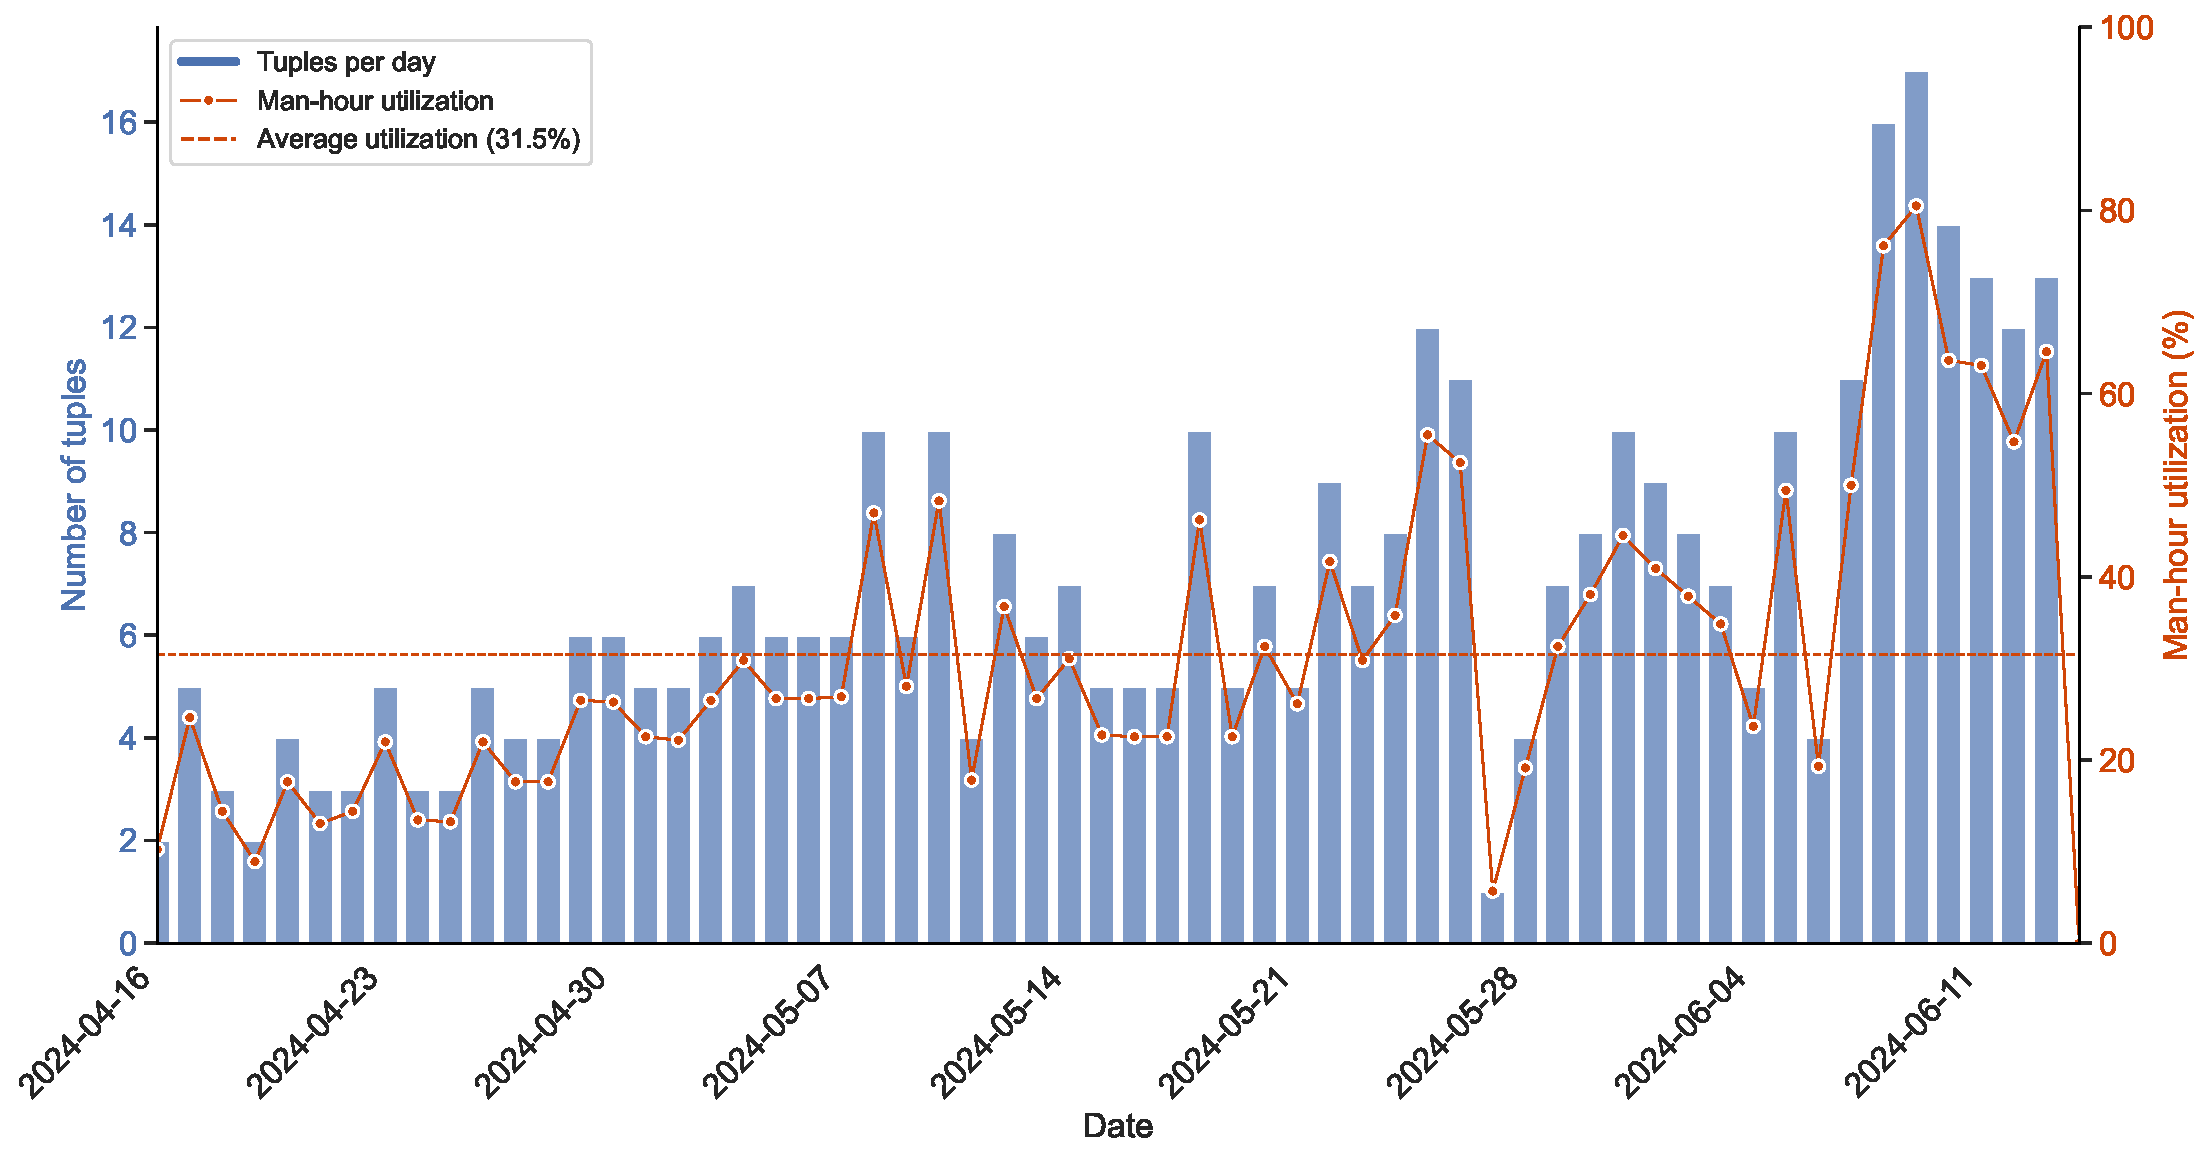
\includegraphics[width=\linewidth]{60_day_check.pdf}
    \caption{Aircraft maintenance scheduling results over a 60-day planning horizon}
    \label{fig:60_day_planning_horizon}
\end{figure}

Figure~\ref{fig:dtg_distribution} presents the distribution of the DTG on the day of maintenance for each scheduled tuple. When a tuple is scheduled for maintenance on the latest possible day, i.e., with a DTG of 1, a 100\% yield can be achieved (i.e., no useful days are wasted). It can be seen that zero waste can be achieved for 83.6\% of the scheduled tuples. Other tuples are scheduled for maintenance prematurely. In other words, a tuple is scheduled for maintenance before its due date mainly due to capacity constraints.

\begin{figure}[htbp]
    \centering
    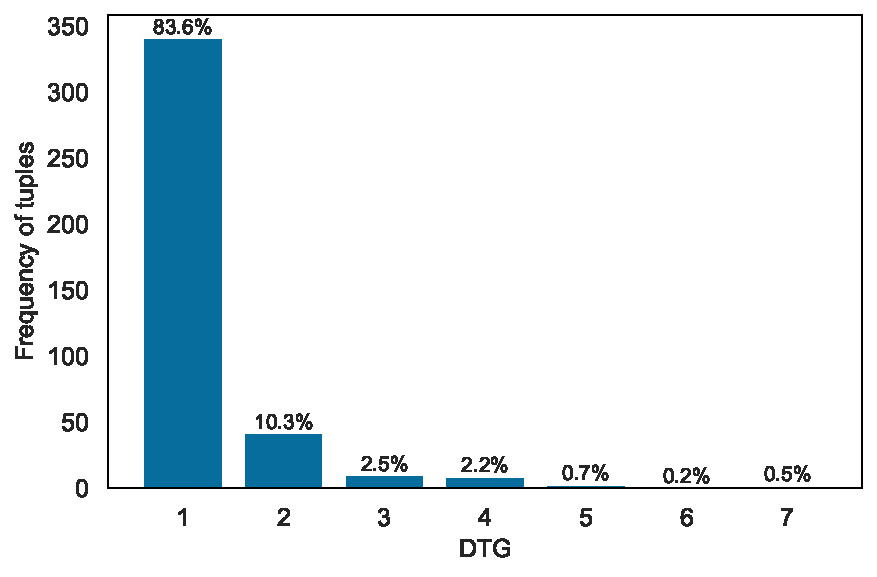
\includegraphics[width=0.6\linewidth]{dtg_hist.pdf}
    \caption{Distribution of resulting DTG on the maintenance day}
    \label{fig:dtg_distribution}
\end{figure}

Figure~\ref{fig:tuples_stat} first shows the distribution of scheduled tuples by check type. Over half of the scheduled tuples are A checks, while the rest are One-C or Two-C checks. This distribution is understandable, as A checks have a relatively short maintenance interval, and One-C checks need to be conducted more frequently than Two-C checks. Regarding C checks, we note that one or two phase checks can be scheduled for one aircraft on a day. The optimization results indicate that in 7.2\% of the cases, Two-C checks are conducted for an aircraft on the same day. Figure~\ref{fig:tuples_stat} further shows the distribution of these scheduled tuples across maintenance stations. Notably, Stations 17 and 31 accommodate a large number of A checks only without serving any phase checks due to their capabilities. The number of scheduled tuples per station ranges from less than 10 to over 50.


\begin{figure}[htbp]
    \centering    
    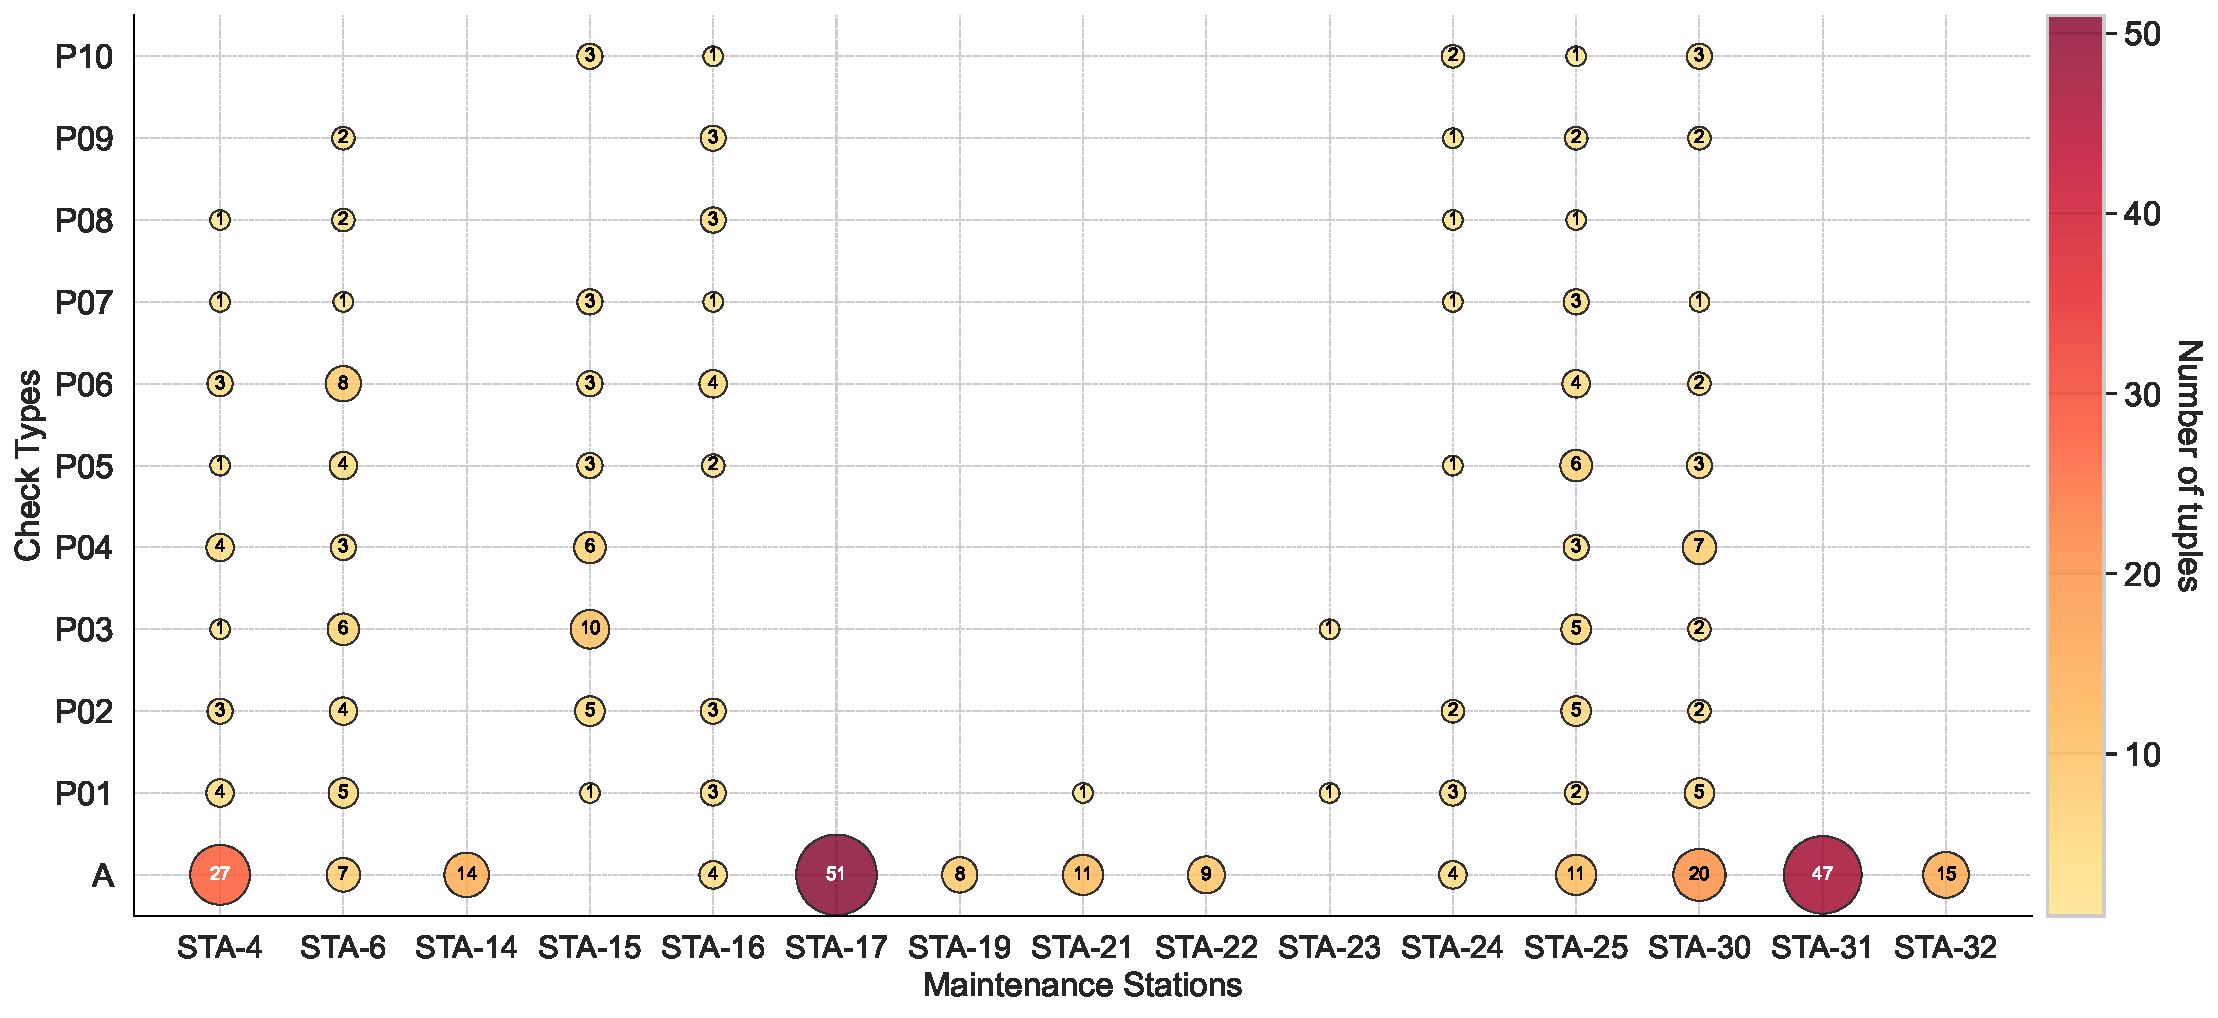
\includegraphics[width=\linewidth]{check_a_sta.pdf}
    \caption{Distribution of scheduled checks over check types and maintenance stations}
    \label{fig:tuples_stat}
\end{figure}


After analyzing the optimization results, we examine the computation time. For the 60-day planning horizon, the total computation time is 421 seconds. We next increase the planning horizon length and observe how the computation time increases accordingly in Table~\ref{tab:increase_tuple}. Note that a longer planning horizon also implies more tuples for planning, as well as more variables and constraints. It can be observed that as the planning horizons $|T|$ increase, the solution time increases exponentially. For the 100-day planning horizon, we could not achieve an optimal solution within the time limit of 7,200 seconds, although the final optimality gap is 0.76\%, provided by the solver. Note that when $|T| = 100$, the resulting integer program has over three million constraints and one million variables.




\begin{table}[htbp]
\centering
\caption{Effect of planning horizon length $|T|$ on computation time}
\label{tab:increase_tuple}
\resizebox{0.8\columnwidth}{!}{%
\begin{tabular}{@{}ccccc@{}}
\toprule
\textbf{$|T|$} & Number of tuples & Number of constraints & Number of variables & Time (secs) \\ \midrule
50 & 462 & 741,248 & 371,150 & 204 \\
60 & 567 & 1,098,688 & 559,020 & 421 \\
70 & 699 & 1,569,144 & 821,240 & 782 \\
80 & 818 & 2,061,026 & 1,098,000 & 1,986 \\
90 & 934 & 2,596,364 & 1,407,780 & 3,942 \\
100 & 1053 & 3,219,916 & 1,772,000 &$>$7,200 \\ \bottomrule 
\end{tabular}%
}
\end{table}



\subsection{Joint Problem Optimization Results under Capacity Reductions}
\label{subsection:jp_resultReducedCap}
In Section~\ref{subsection:jp_result}, all 15 maintenance stations are available. We next explore how optimization results would differ when some stations are unavailable. Each of the 15 stations can accommodate one A check daily while the number of phase checks $U_j$ differs. Depending on how many phase checks a station can accommodate daily, we divide 15 stations into three categories: (i) six stations cannot accommodate any phase checks ($U_j = 0$); (ii) seven stations can accommodate one phase check daily ($U_j = 1$); and (iii) two stations can accommodate two phase checks daily ($U_j = 2$). We then design the following capacity reduction scenarios, shown in Table \ref{tab:capacity_reduction}. In each scenario, the number of stations is reported by category, along with the capacity limits.

\begin{table}[htbp]
\centering
\caption{Capacity reduction scenarios}
\label{tab:capacity_reduction}
\resizebox{\columnwidth}{!}{%
\begin{tabular}{@{}cccccccc@{}}
\toprule
Scenario & Category (i) & Category (ii) & Category (iii) & Total \# of stations & A check limit & Phase check limit & MH limit \\ \midrule
1 & 6 & 7 & 2 & 15 & 15 & 11 & 2,112 \\
2 & 5 & 5 & 2 & 12 & 12 & 9 & 1,704 \\
3 & 4 & 4 & 2 & 10 & 10 & 8 & 1,464 \\
4 & 4 & 4 & 1 & 9 & 9 & 6 & 1,224 \\
5 & 3 & 3 & 1 & 7 & 7 & 5 & 984
\\ \bottomrule
\end{tabular}%
}
\end{table}


 

\begin{figure}[htbp]
    \centering
     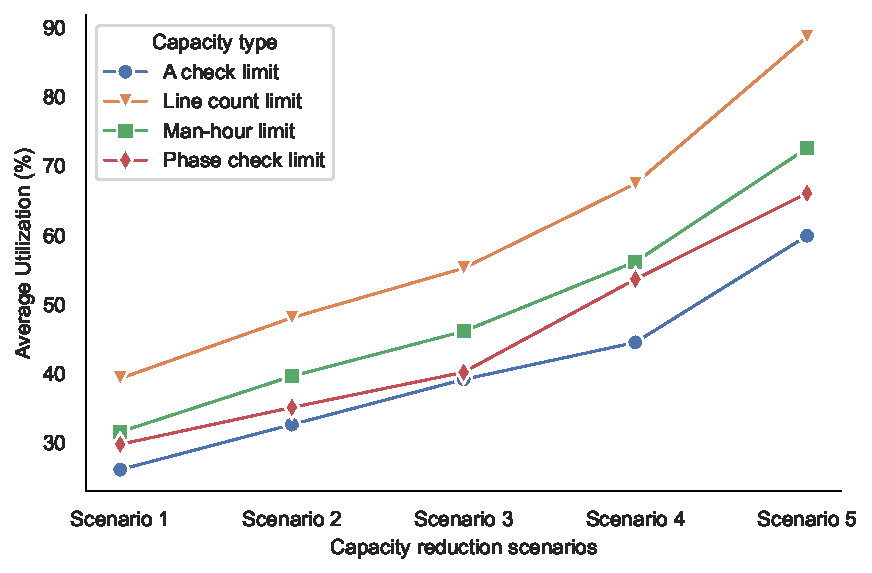
\includegraphics[width=0.7\linewidth]{utilization_v1.pdf}
    \caption{Capacity utilization ratios under different scenarios}
    \label{fig:impact_utilization}
\end{figure}

We resolve the joint problem under each capacity reduction scenario using the same 60-day planning period. Instead of presenting detailed optimization results under each scenario, Figure~\ref{fig:impact_utilization} shows the average capacity utilization over all applicable stations and over time for each capacity type. The A check capacity utilization ratio is calculated as $\left(\sum_{j \in J}\sum_{w \in \bar{W}}x_{wj}^t\right) /\sum_{j \in J}\bar{A}_j^t$. Similarly, the phase check capacity utilization ratio is $\left(\sum_{j \in J}\sum_{w \in \hat{W}\cup\breve{W}}x_{wj}^t\right) /\sum_{j \in J}\bar{U}_j^t$ and the line count utilization ratio is $\left(\sum_{j \in J}\sum_{i \in I}z_{ij}^t\right) /\sum_{j \in J}\bar{Q}_j^t$. It is clear that as the number of available stations drops, i.e., the amount of available capacity drops, the capacity utilization for each capacity type increases consequentially, since the maintenance demand is fixed. Notably, the line count (the number of distinct aircraft a station can handle) has the highest average utilization, which is nearly 90\% in Scenario 5.

Understandably, for the same maintenance demand, reducing the number of available maintenance stations leads to premature maintenance due to an increasing likelihood of having binding capacity constraints. 


\begin{figure}
    \centering
    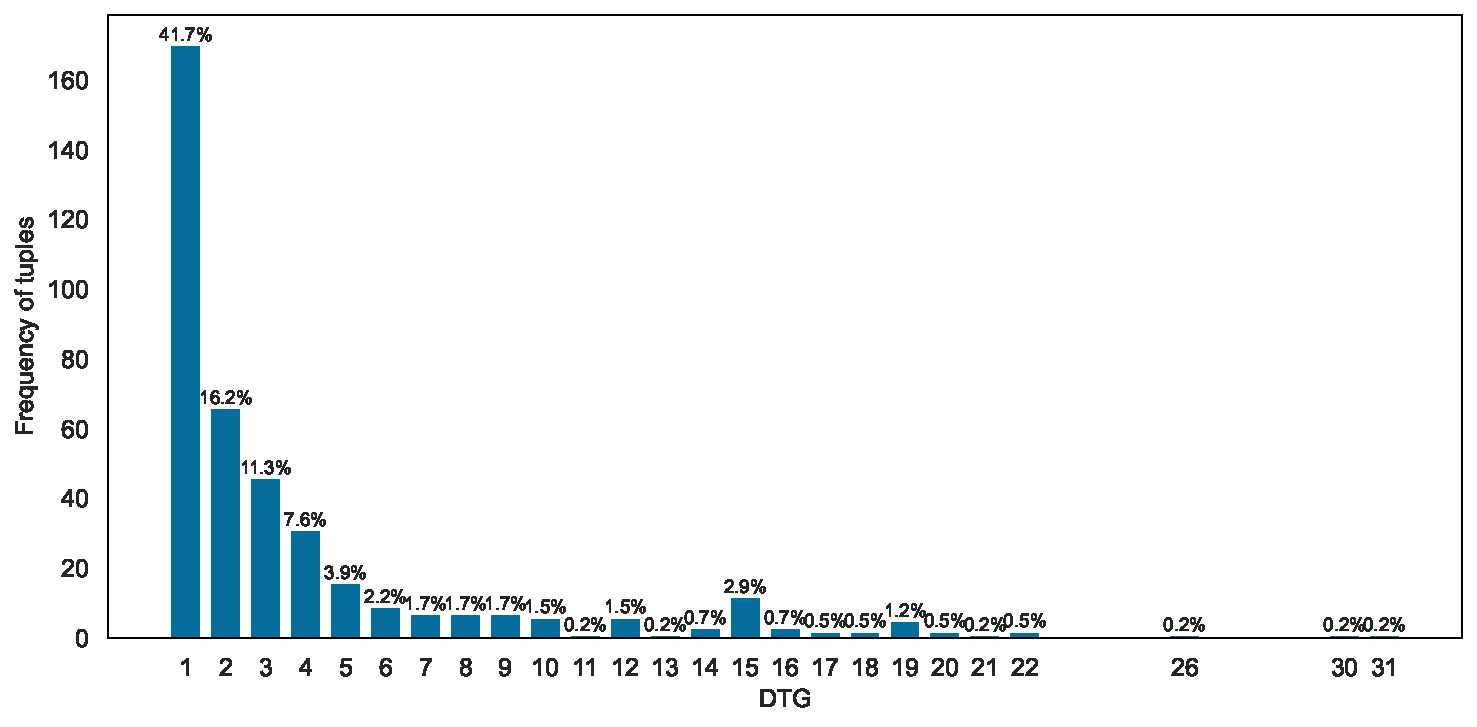
\includegraphics[width=\linewidth]{dtg_hist_s5.pdf}
    \caption{Distribution of resulting DTG on the maintenance day under Scenario 5}
    \label{fig:scenario5DTG}
\end{figure}

Figure~\ref{fig:scenario5DTG} shows the resulting distribution of DTGs on the day of maintenance under Scenario 5. As compared with Figure~\ref{fig:dtg_distribution}, fewer tuples can achieve a 100\% yield (i.e., zero waste) when the capacity is substantially reduced. We also note that reducing the number of maintenance stations results into a higher optimization objective (discounted maintenance cost).



\begin{table}[htbp]
\centering
\caption{Effect of capacity reductions on computation time }
\label{tab:my-cap-reduction-time}
\resizebox{0.8\columnwidth}{!}{%
\begin{tabular}{@{}ccccc@{}}
\toprule
\multicolumn{1}{l}{Scenario} & Number of stations & Number of constraints & Number of variables & Time (secs) \\ \midrule
1 & 15 & 1,098,688 & 559,020 & \textbf{421} \\
2 & 12 & 917,848 & 447,540 & 431 \\
3 & 10 & 795,328 & 361,860 & 495 \\
4 & 9 & 740,488 & 331,860 & 513 \\
5 & 7 & 640,168 & 301,740 & 6,086 \\ \bottomrule
\end{tabular}%
}
\end{table}


Table~\ref{tab:my-cap-reduction-time} shows that as the number of available stations decreases, the computation time increases. Note that the computation time of 421 seconds under the full-capacity scenario is reported earlier in Table~\ref{tab:increase_tuple}. Hence, with fewer stations, the joint optimization becomes more constrained with limiting flexibility in scheduling and assignment decisions.  Although the numbers of variables and constraints reduce, it is increasingly difficult to find feasible planning decisions due to increasingly tight capacity constraints, which indirectly leads to increased computational time. 

\subsection{Performance of Decomposition-Based Solution Approaches}
\label{performance_decomp}


Section~\ref{subsection:jp_result} has demonstrated that directly solving the JP (i.e., benchmark approach) is impractical when $|T|$ is large. Section~\ref{subsection:jp_resultReducedCap} further shows that the computation time also increases dramatically when few maintenance stations are available. As no other studies have addressed the joint scheduling and station assignment decisions, we cannot compare the two decomposition-based solution approaches with any existing algorithms. Instead, both proposed solution approaches are benchmarked with directly solving the JP with a commercial solver Gurobi. \color{black} Therefore, we next evaluate the performance of two proposed decomposition-based approaches, namely SH described in Section~\ref{sec:SchedulingThenAssign} and TD described in Section~\ref{sec:tempDecomp}. 

Figure~\ref{fig:comparisonS1} compares three solution approaches by the total computation time and the optimization objective under the full capacity scenario, namely Scenario 1. First, both decomposition approaches, i.e., SH and TD, can reduce the computation time by over 80\% when $|T|$ = 100. Second, the weighted maintenance cost increases remain small across the planning horizons, which are less than 0.4\%. Figure~\ref{fig:comparisonS1} also shows that as the planning horizon length grows, the computation time grows nonlinearly while the optimization objective value grows almost in a linear manner. The linear relationship between the optimization objective and the planning horizon length is expected:~for the same aircraft fleet with predetermined maintenance requirements, the total maintenance cost grows linearly with time. \color{black} By contrast, Figure~\ref{fig:comparisonS4} presents a similar comparison while under Scenario 4. While the weighted cost increases are larger, they are below 2\%, remaining small. Therefore, both decomposition approaches strike a much more preferable tradeoff between solution time and quality. Specifically, the proposed decomposition approaches can reduce the computation time by 80\% while increasing the objective value by less than 2\%.

\begin{figure}[htbp]
    \centering
    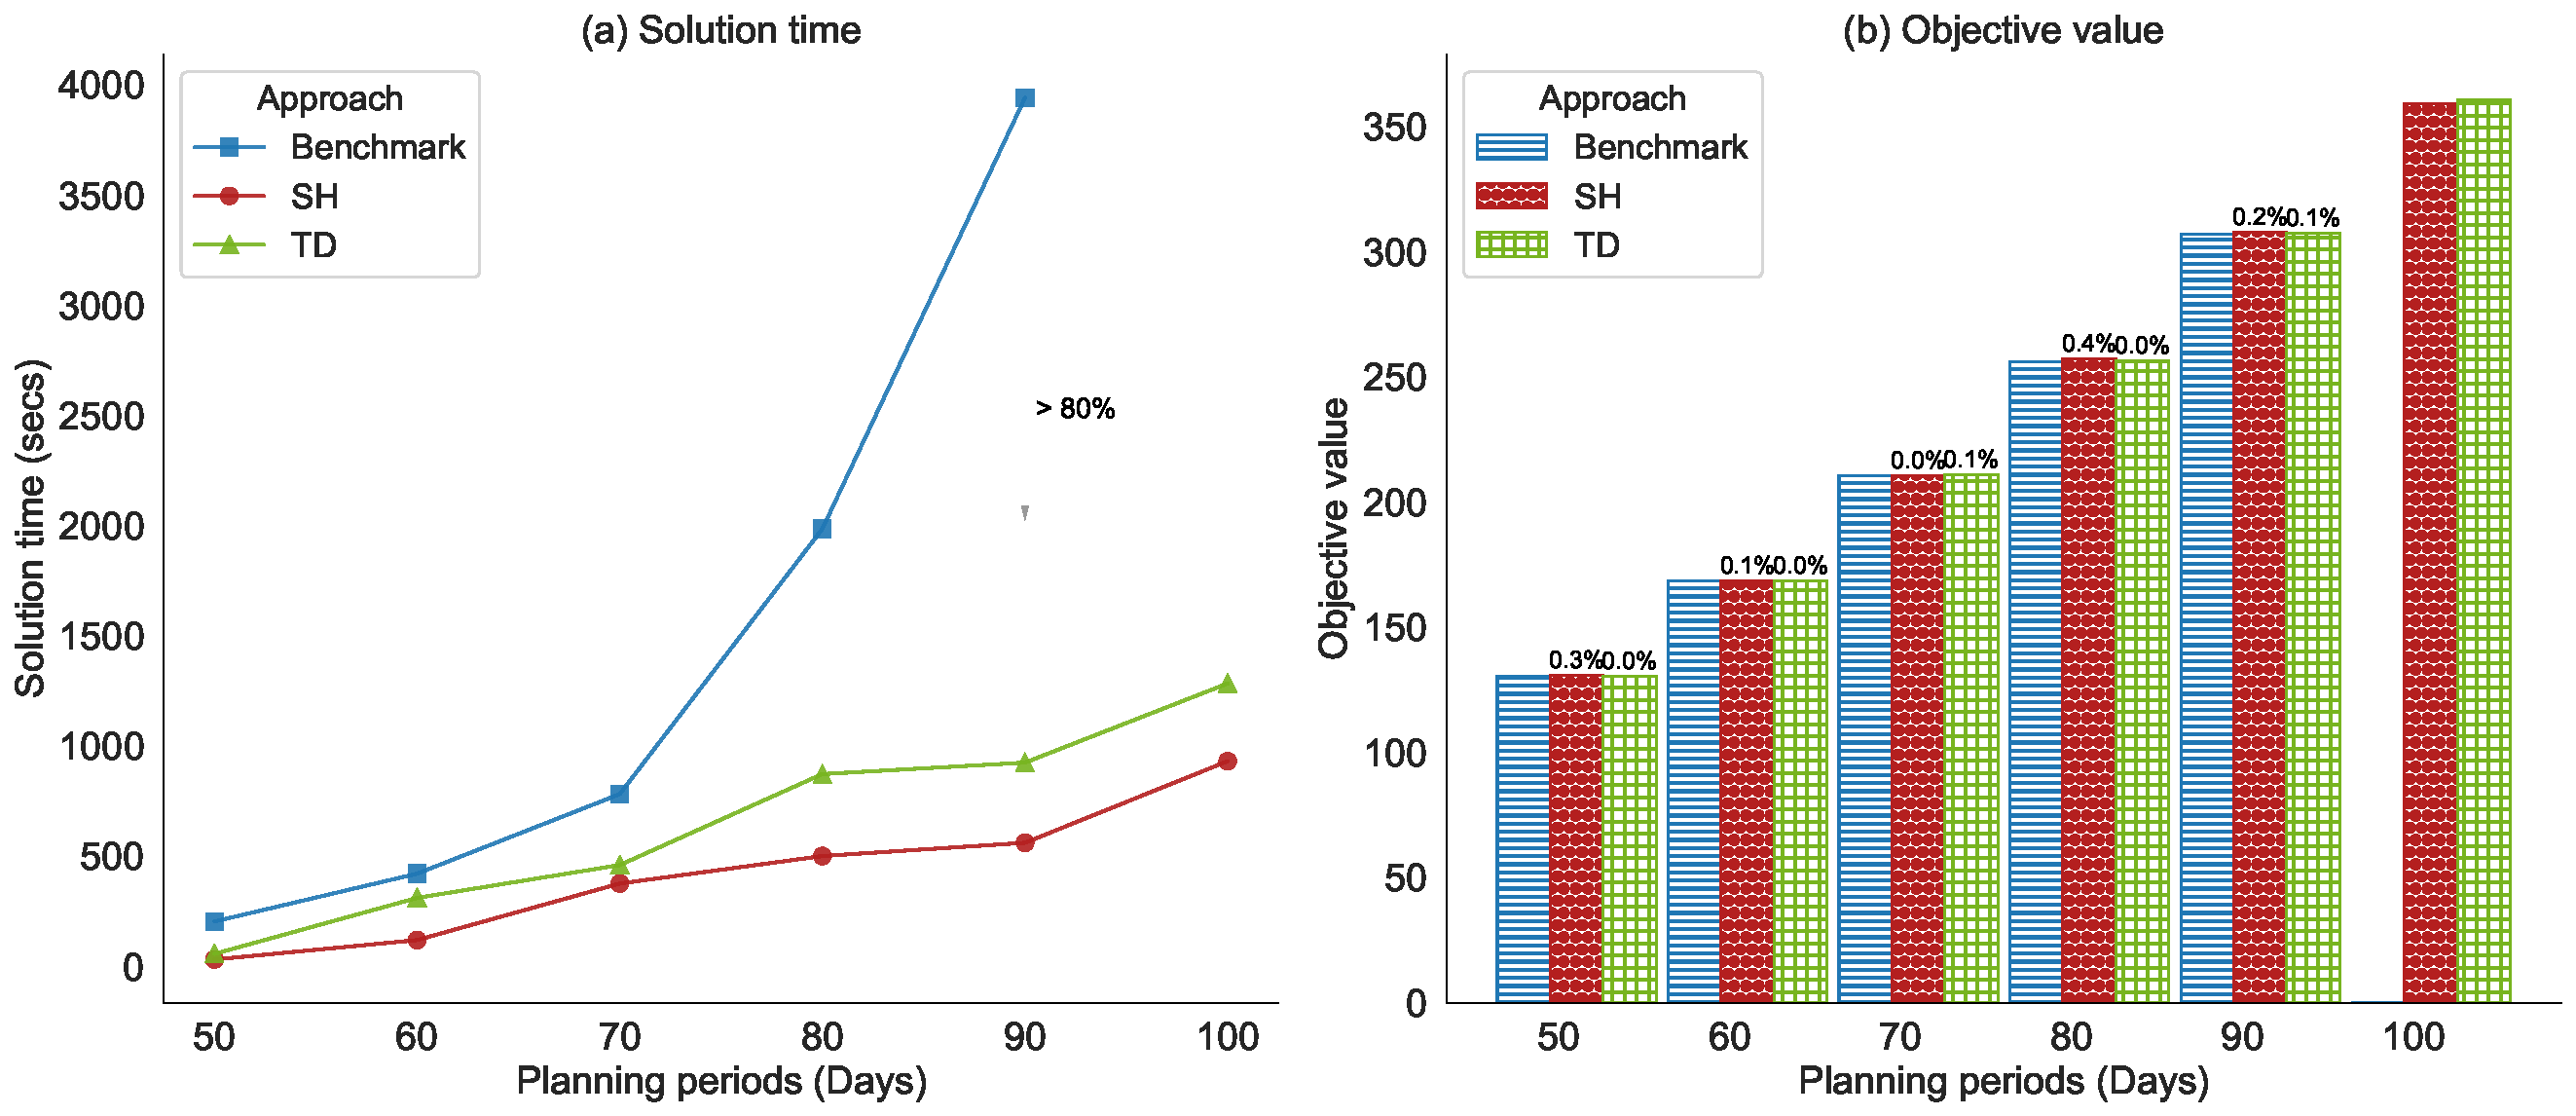
\includegraphics[width=\linewidth]{comb_compS1_v1.pdf}
    \caption{Comparison of three solution approaches under Scenario 1}
    \label{fig:comparisonS1}
\end{figure}

\begin{figure}[htbp]
    \centering
    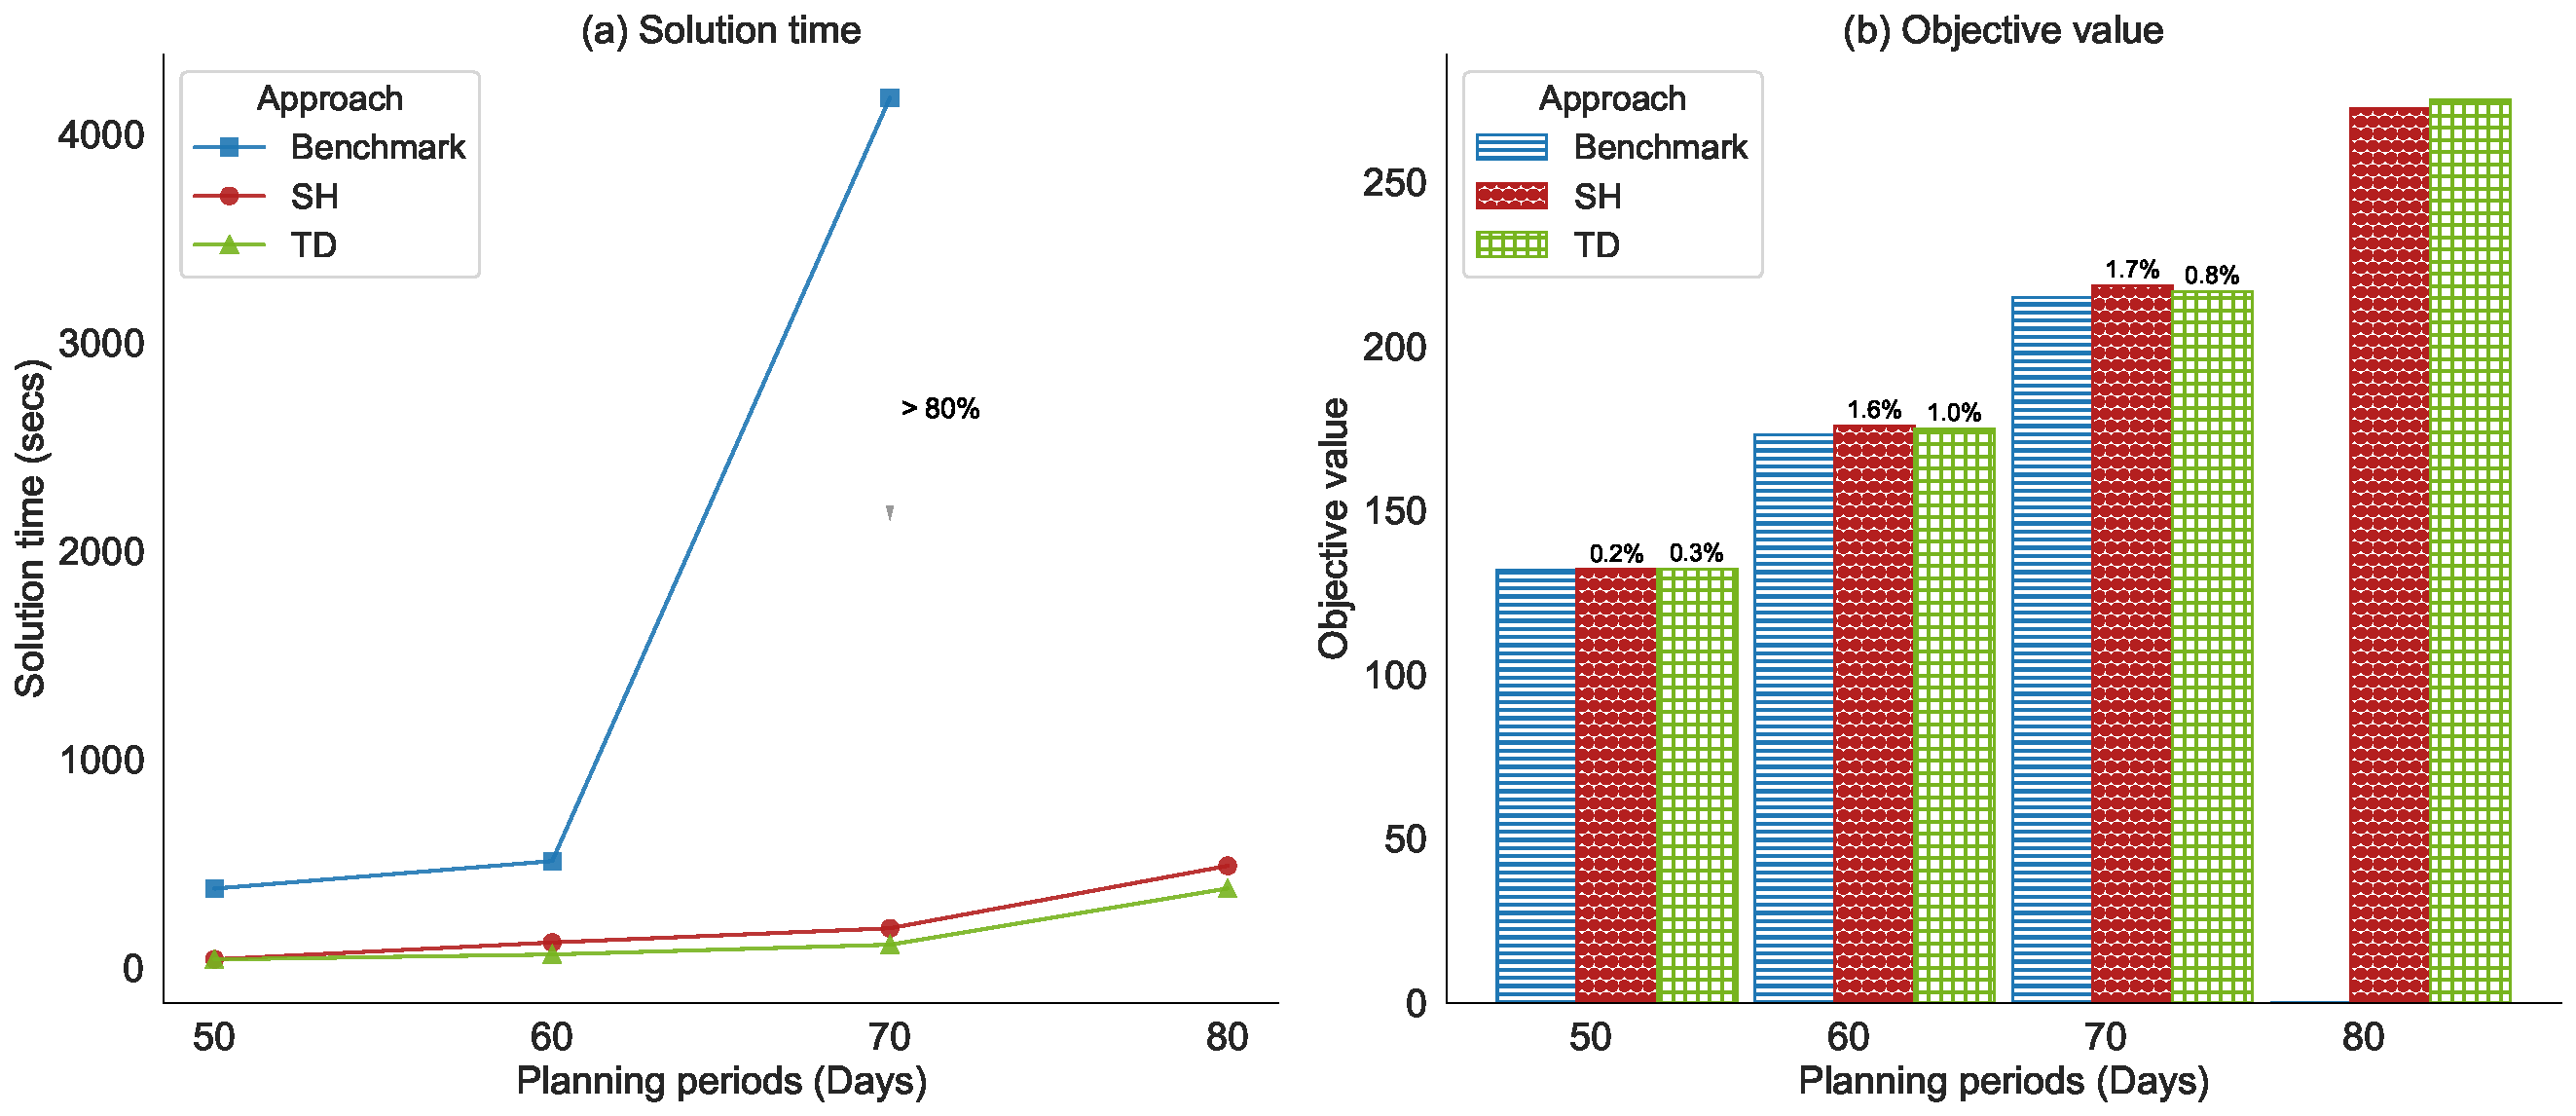
\includegraphics[width=\linewidth]{comb_compS4_v1.pdf}
    \caption{Comparison of three solution approaches under Scenario 4}
    \label{fig:comparisonS4}
\end{figure}


We next explain why the relative difference in the optimization objective seems very little, first with a toy example. Assume that there is a single tuple for maintenance at the only station. The optimal decision is to schedule it for day $t\prime$ and an alternative decision is to have the maintenance on day $t\prime-n$. The absolute cost difference due to the premature scheduling is $\gamma^{t\prime-n} - \gamma^{t\prime}$ and the relative cost change is given by $\frac{1}{\gamma^n} - 1$. Assuming $\gamma = 0.99$, the relative difference is 1.0\% when $n = 1$ and 5.2\% when $n = 5$. Similarly, in case of multiple tuples, when each tuple is scheduled one day earlier, the relative cost difference is about 1.0\%. However, one useful day from the previous check could be worth hundreds of or even thousands of dollars. AA is thus interested in comparing solutions in terms of useful day losses. 

We next introduce two concepts for a tuple $w$, namely schedule deviation $\xi_w$ and normalized schedule deviation $\bar{\xi}_w$. $\xi_w$ is computed as follows:
\begin{equation}
    \xi_w =  t_w - t_w^*, \quad \forall w \in W,
\end{equation}
where $t_w^*$ is the optimum maintenance day for tuple $w$ and $t_w$ is an alternative day suggested by a heuristic approach. Clearly, when two approaches schedule a tuple on the same day (i.e.,  $t_w = t_w^*$), the scheduling deviation is stated to be zero; further, when $t_w < t_w^*$, the scheduling difference is stated to be negative (premature maintenance); when $t_w > t_w^*$ the scheduling deviation is positive (delayed maintenance). Note even when a heuristic produces a delayed maintenance decision, the maintenance is not overdue (i.e., the minimum DTW is greater than 0). When we further consider the tuple-specific maintenance interval $m_w$, the scheduled deviation can be normalized as follows:
\begin{equation}
    \bar{\xi}_w =  \frac{t_w - t_w^*}{m_w}, \quad \forall w \in W.
\end{equation}

We next focus on the 70-day planning horizon under Scenario 4. First, all three approaches, i.e., benchmark, SH, and TD, have yielded the same number of scheduled tuples over the planning horizon. However, the maintenance schedules are different.

Figure~\ref{fig:sched_deviation} shows $t_w^*$ and $t_w$ for each scheduled tuple for both the SH and TD approaches. As multiple tuples could be scheduled on the same day, the size of each point in Figure~\ref{fig:sched_deviation} indicates the number of tuples. In other words, one point corresponds to one or multiple scheduled tuples. We can observe that most points fall either on the 45-degree line (i.e., indicating no schedule deviations) or lie close to the 45-degree line, indicating little schedule deviations. Additionally, Figure~\ref{fig:normalized_dev} shows the distribution of the normalized schedule deviation $\bar{\xi}_w$. Although $\bar{\xi}_w$ varies dramatically from -70\% to +100\%, for over 96\% of the tuples, $\bar{\xi}_w$ is within a small range, namely $-10\%$ and $+10\%$, regardless of the solution approach (SH or TD).


\begin{figure}[htbp]
    \centering
    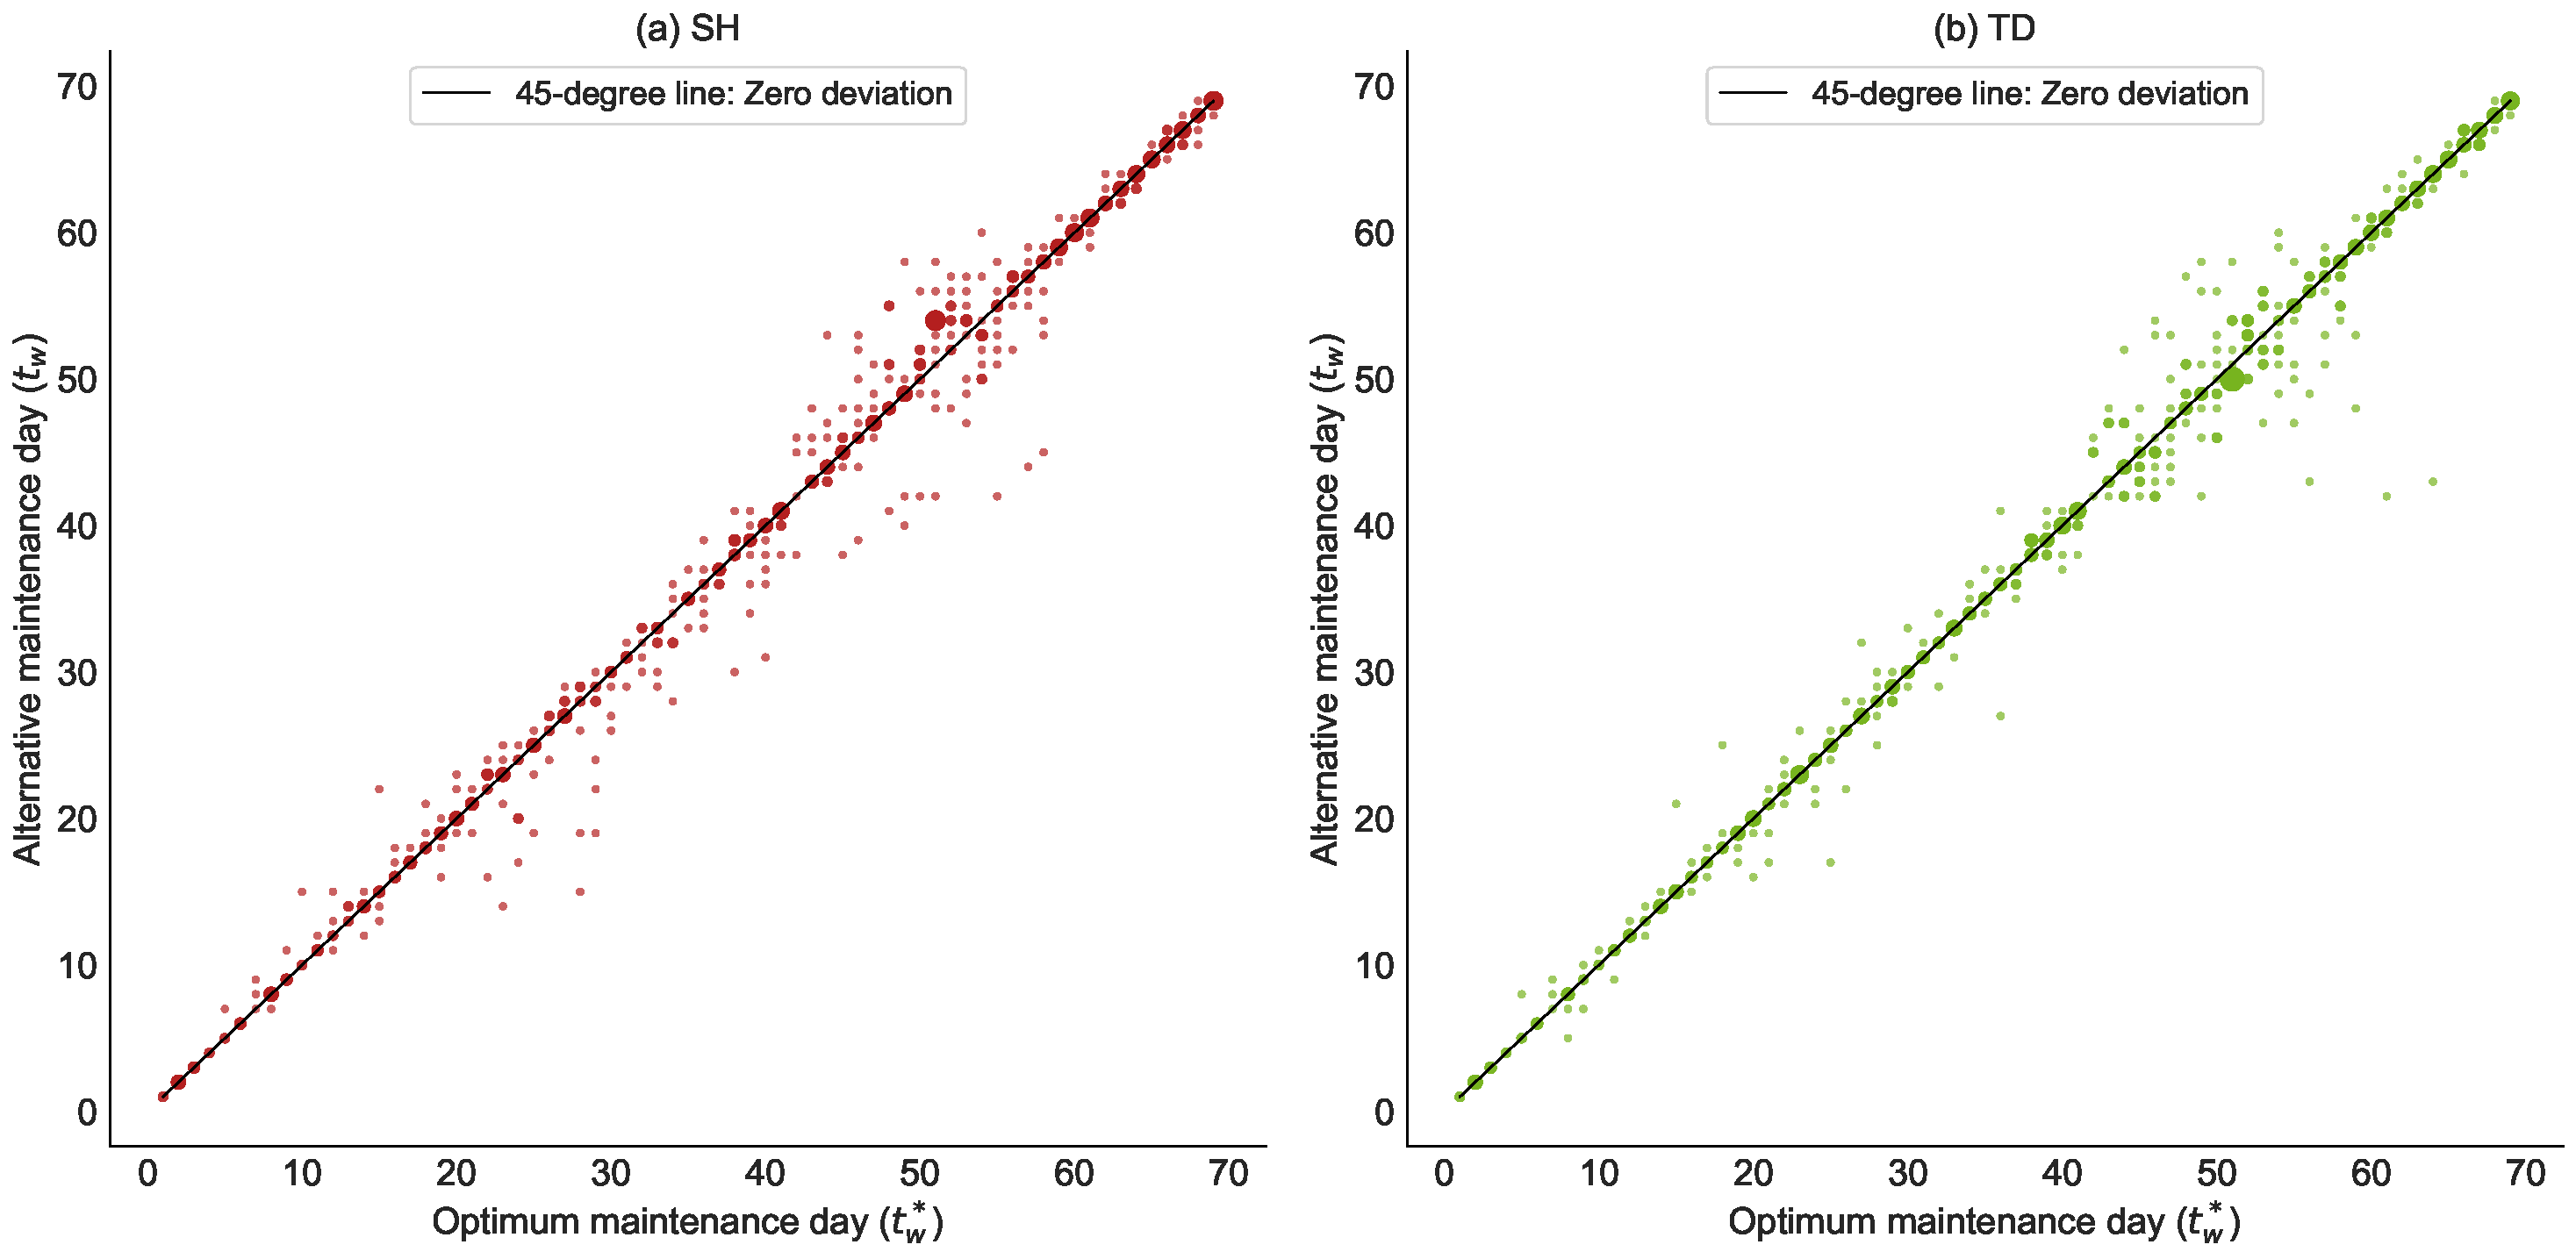
\includegraphics[width=\linewidth]{sched_dev_70.pdf}
    \caption{Scheduled deviations ($\xi_w$) for the 70-day planning horizon under Scenario 4}
    \label{fig:sched_deviation}
\end{figure}

\begin{figure}[htbp]
    \centering
    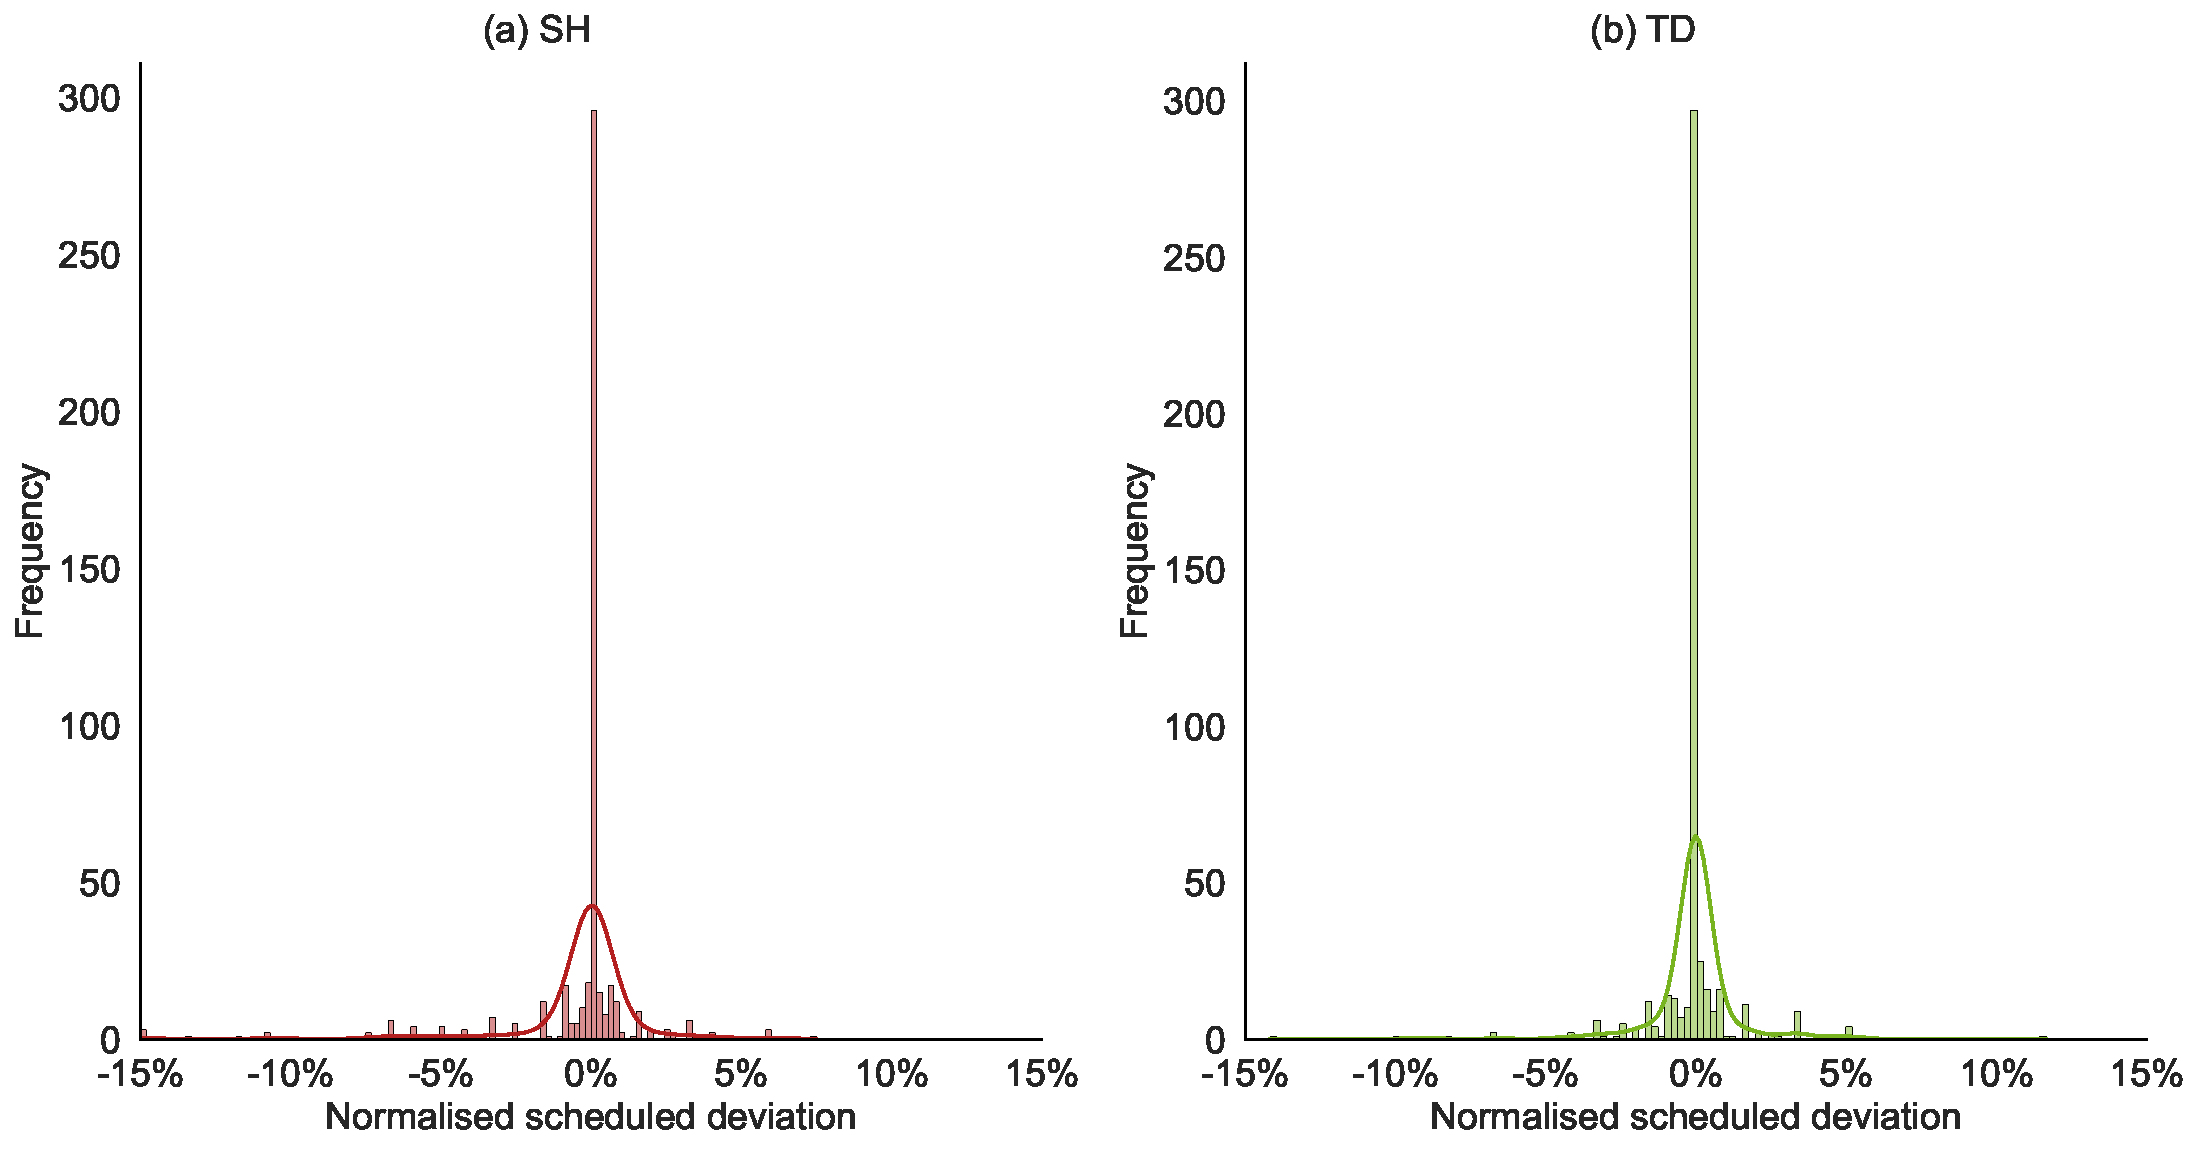
\includegraphics[width=\linewidth]{normalise_dev.pdf}
    \caption{Distribution of $\bar{\xi}_w$ for 70-day planning horizon  under Scenario 4}
    \label{fig:normalized_dev}
\end{figure}

% \begin{figure}[htbp]
%     \centering
%     \includegraphics[width=0.8\linewidth]{sched_dev.pdf}
%     \caption{Evaluation of normalized scheduled deviation $\%$ over different planning horizon lengths under scenario 4}
%     \label{fig:overal_schd_dev}
% \end{figure}

% \newpage
\subsection{A Long-term Analysis}
\label{sec:long_termAna}

After validating the high efficiency and capabilities of two decomposition-based solution approaches, we tackle a long-term planning problem. Specifically, TD is used to plan aircraft maintenance activities over a 180-day planning horizon from April 16 to October 12, 2024 assuming all stations are available (i.e., under Scenario 1). 

After pre-processing (i.e., removing tuples with very large DTGs), there are 823 aircraft and 1,631 tuples for scheduling and assignment. After solving the problem, 1,525 tuples have been scheduled, yielding a total number of 1,806 checks because a tuple could be scheduled multiple times for maintenance over the 180-day horizon. Figure~\ref{fig:schd_pertuple} shows that among 1,525 tuples, 218 tuples are scheduled for maintenance more than once (having different scheduled cycles), while the rest (1,307 tuples) are scheduled for maintenance exactly once. Notably, five tuples experience four maintenance cycles over the 180-day period. Figure~\ref{fig:schd_tuple_cycles} shows maintenance cycles for some selected tuples. Note that those four example tuples are for A checks but involve different aircraft manufacturers. For some Boeing aircraft, A checks are needed every 60 days; for Airbus, the maintenance interval for A checks could be for 120 or 150 days. Additionally, it is quite clear from Figure~\ref{fig:schd_tuple_cycles} that the DTG is not necessarily 1 when a check is scheduled.


\begin{figure}[htbp]
    \centering
    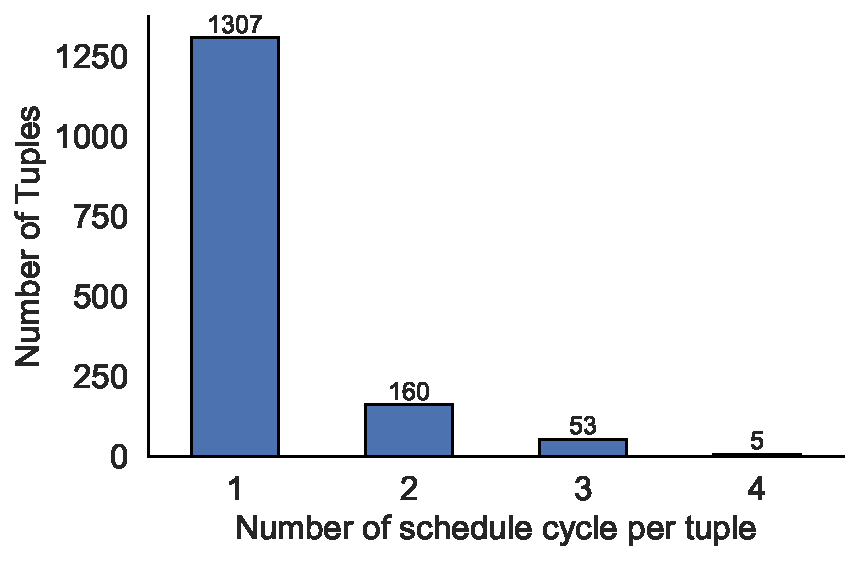
\includegraphics[width=0.5\linewidth]{Num_per_tuples.pdf}
    \caption{Distribution of the number of scheduled cycles per tuple}
    \label{fig:schd_pertuple}
\end{figure}

\begin{figure}[htbp]
    \centering
    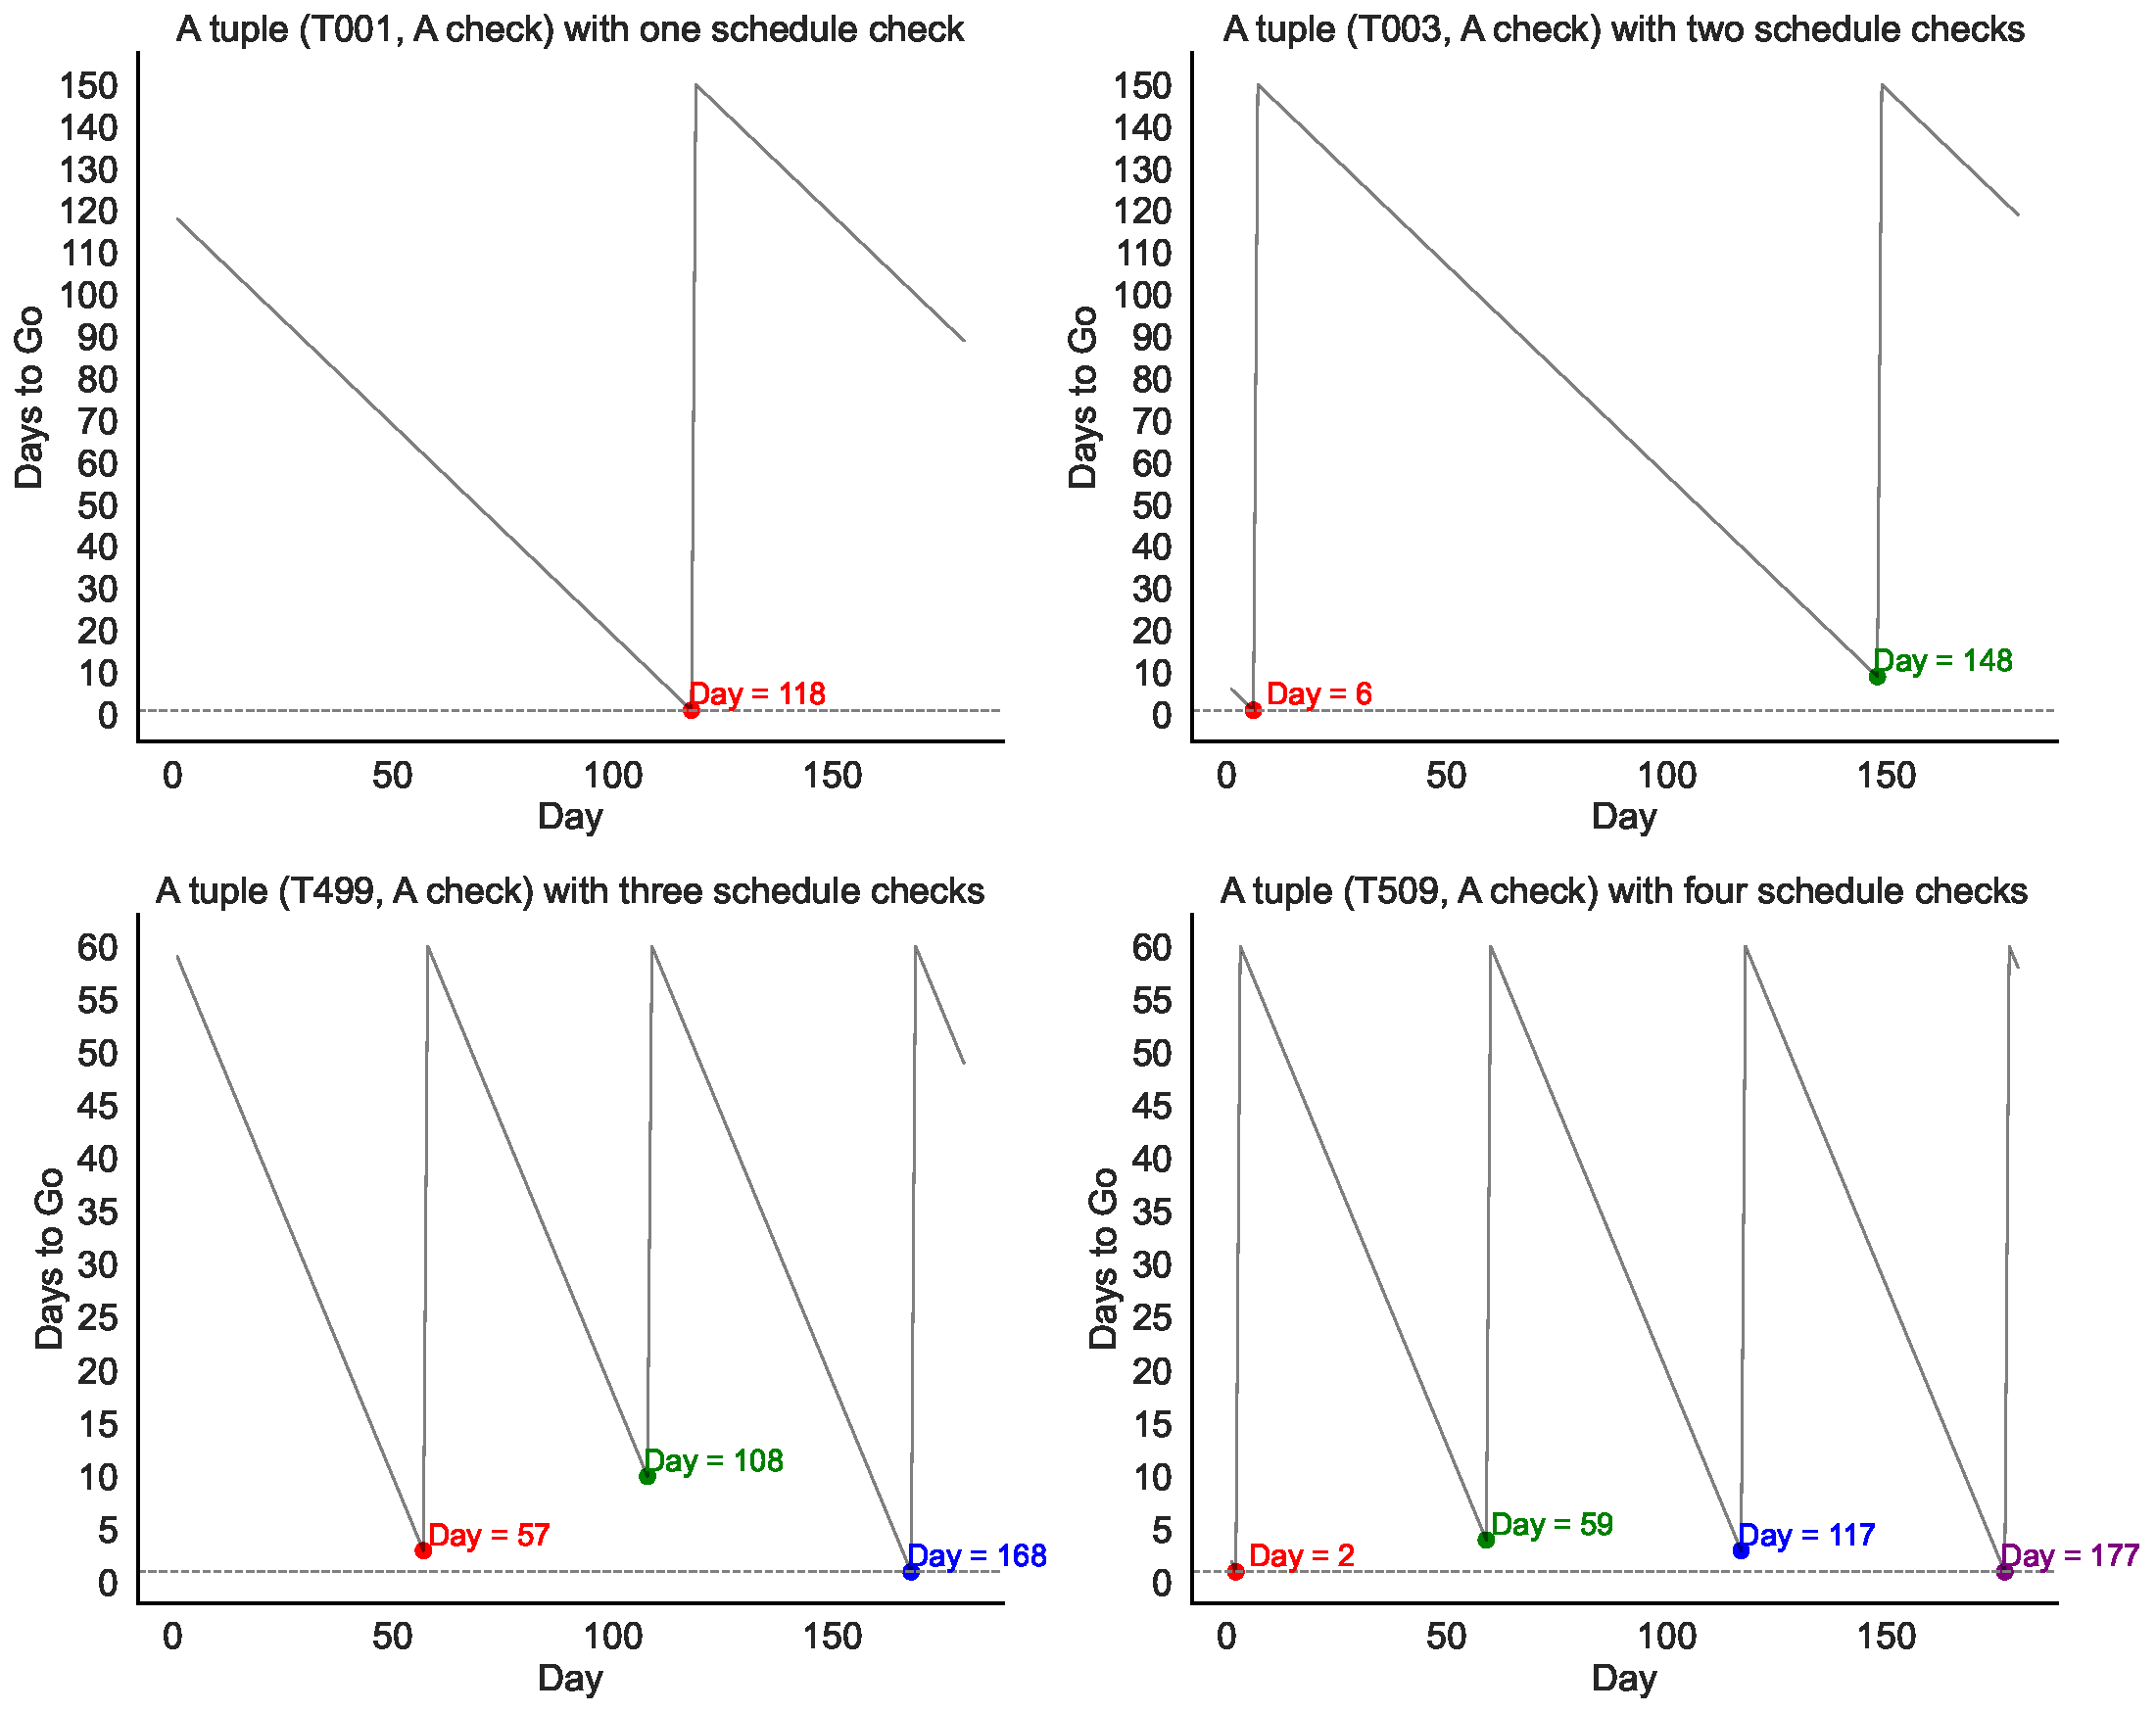
\includegraphics[width=0.9\linewidth]{schd_cycle.pdf}
    \caption{Schedule cycles for some selected tuples }
    \label{fig:schd_tuple_cycles}
\end{figure}


\begin{figure}[htbp]
    \centering
    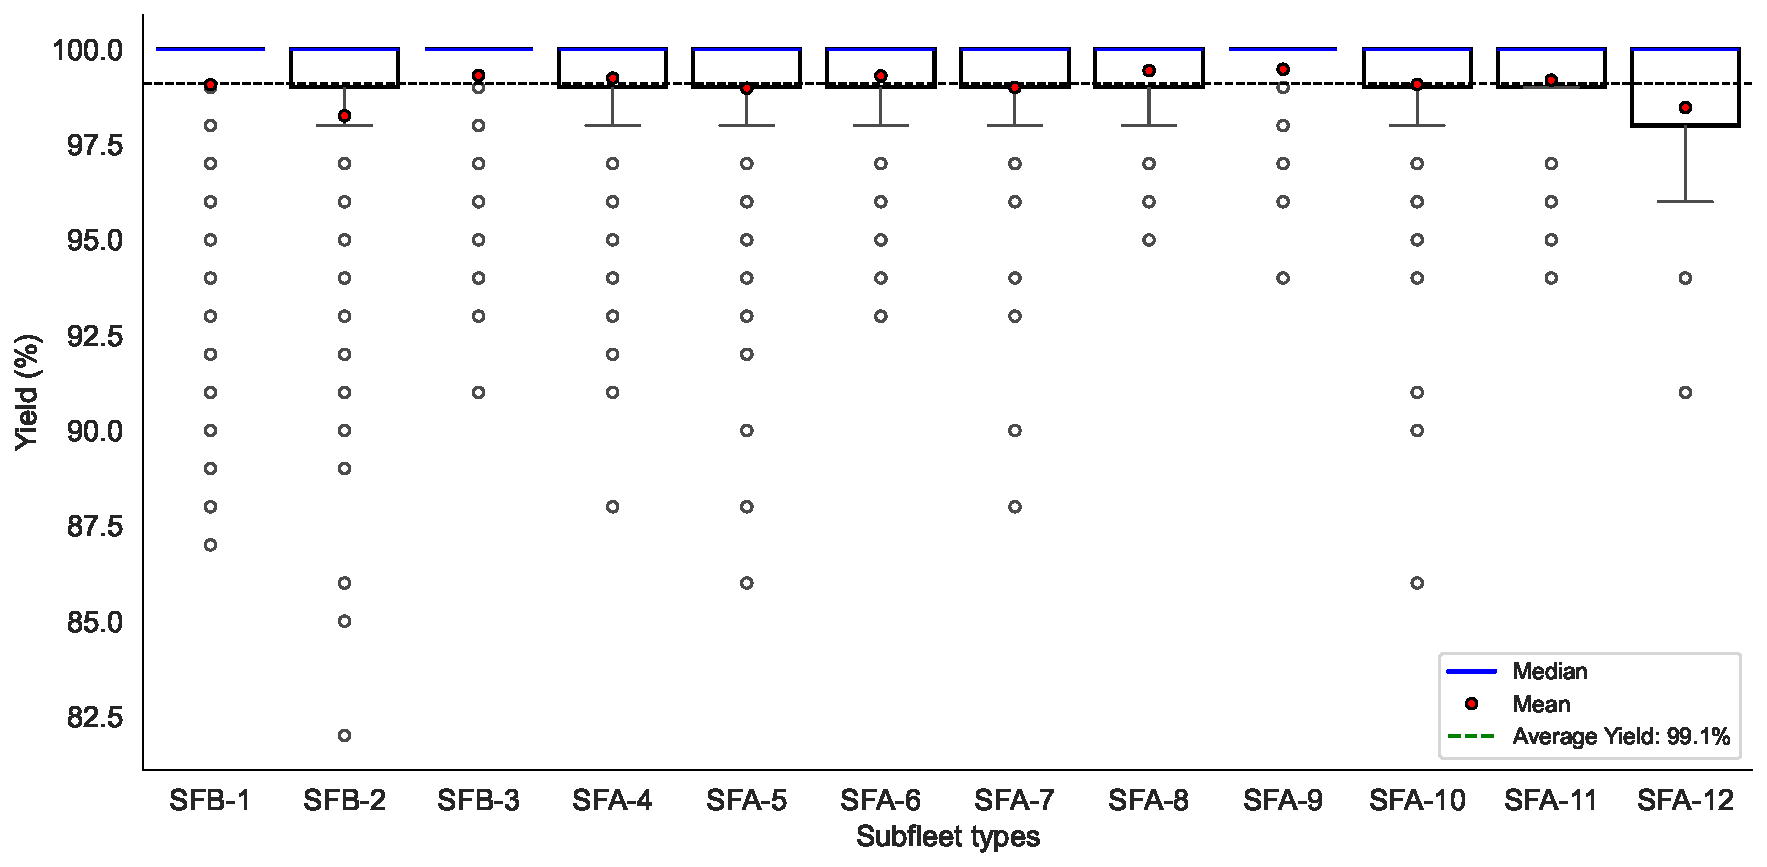
\includegraphics[width=\linewidth]{yields.pdf}
    \caption{Distribution of yield by  subfleet type}
    \label{fig:yieldist}
\end{figure}

Figure~\ref{fig:yieldist} further shows the yield distribution for each subfleet type. Recall that yield is the percentage of useful days being utilized or 100\% minus the percentage of wasted days. Generally, the yield varies from 90\% to 100\%. Note that \cite{yan2008long} explored the same concept of yield, referring to it as the \textit{aircraft use rate}, where an average value of 97.7\% was reported for their case based on a major airport in Taiwan.
Figure~\ref{fig:yieldist} also indicates that the mean variation over various subfleet types is very small, meaning that all subfleet types receive almost equal accommodation over the planning horizon (i.e., no subfleet types are being discriminated).

It is noted that the total computation time for this 180-day analysis is around 1.5 hours.


\subsection{One Application in Aircraft Maintenance Capacity Planning}
\label{sec:twoHolidays}
We next present one application of the developed long-term aircraft maintenance planning model. Specifically, we focus on two major holidays within the 180-day planning horizon: Independence Day and Labor Day. For each holiday, we anticipate a two-week travel period characterized by increased aircraft utilization and nearly no time for conducting maintenance. To model this effect, we reduce the number of aircraft accessing each maintenance station to zero for all subfleet types. In other words, all maintenance stations are effectively shut down and no maintenance activities are scheduled during these periods. We then evaluate how such an adjustment affects maintenance costs during each travel peak period.

\begin{figure}[htbp]
    \centering
    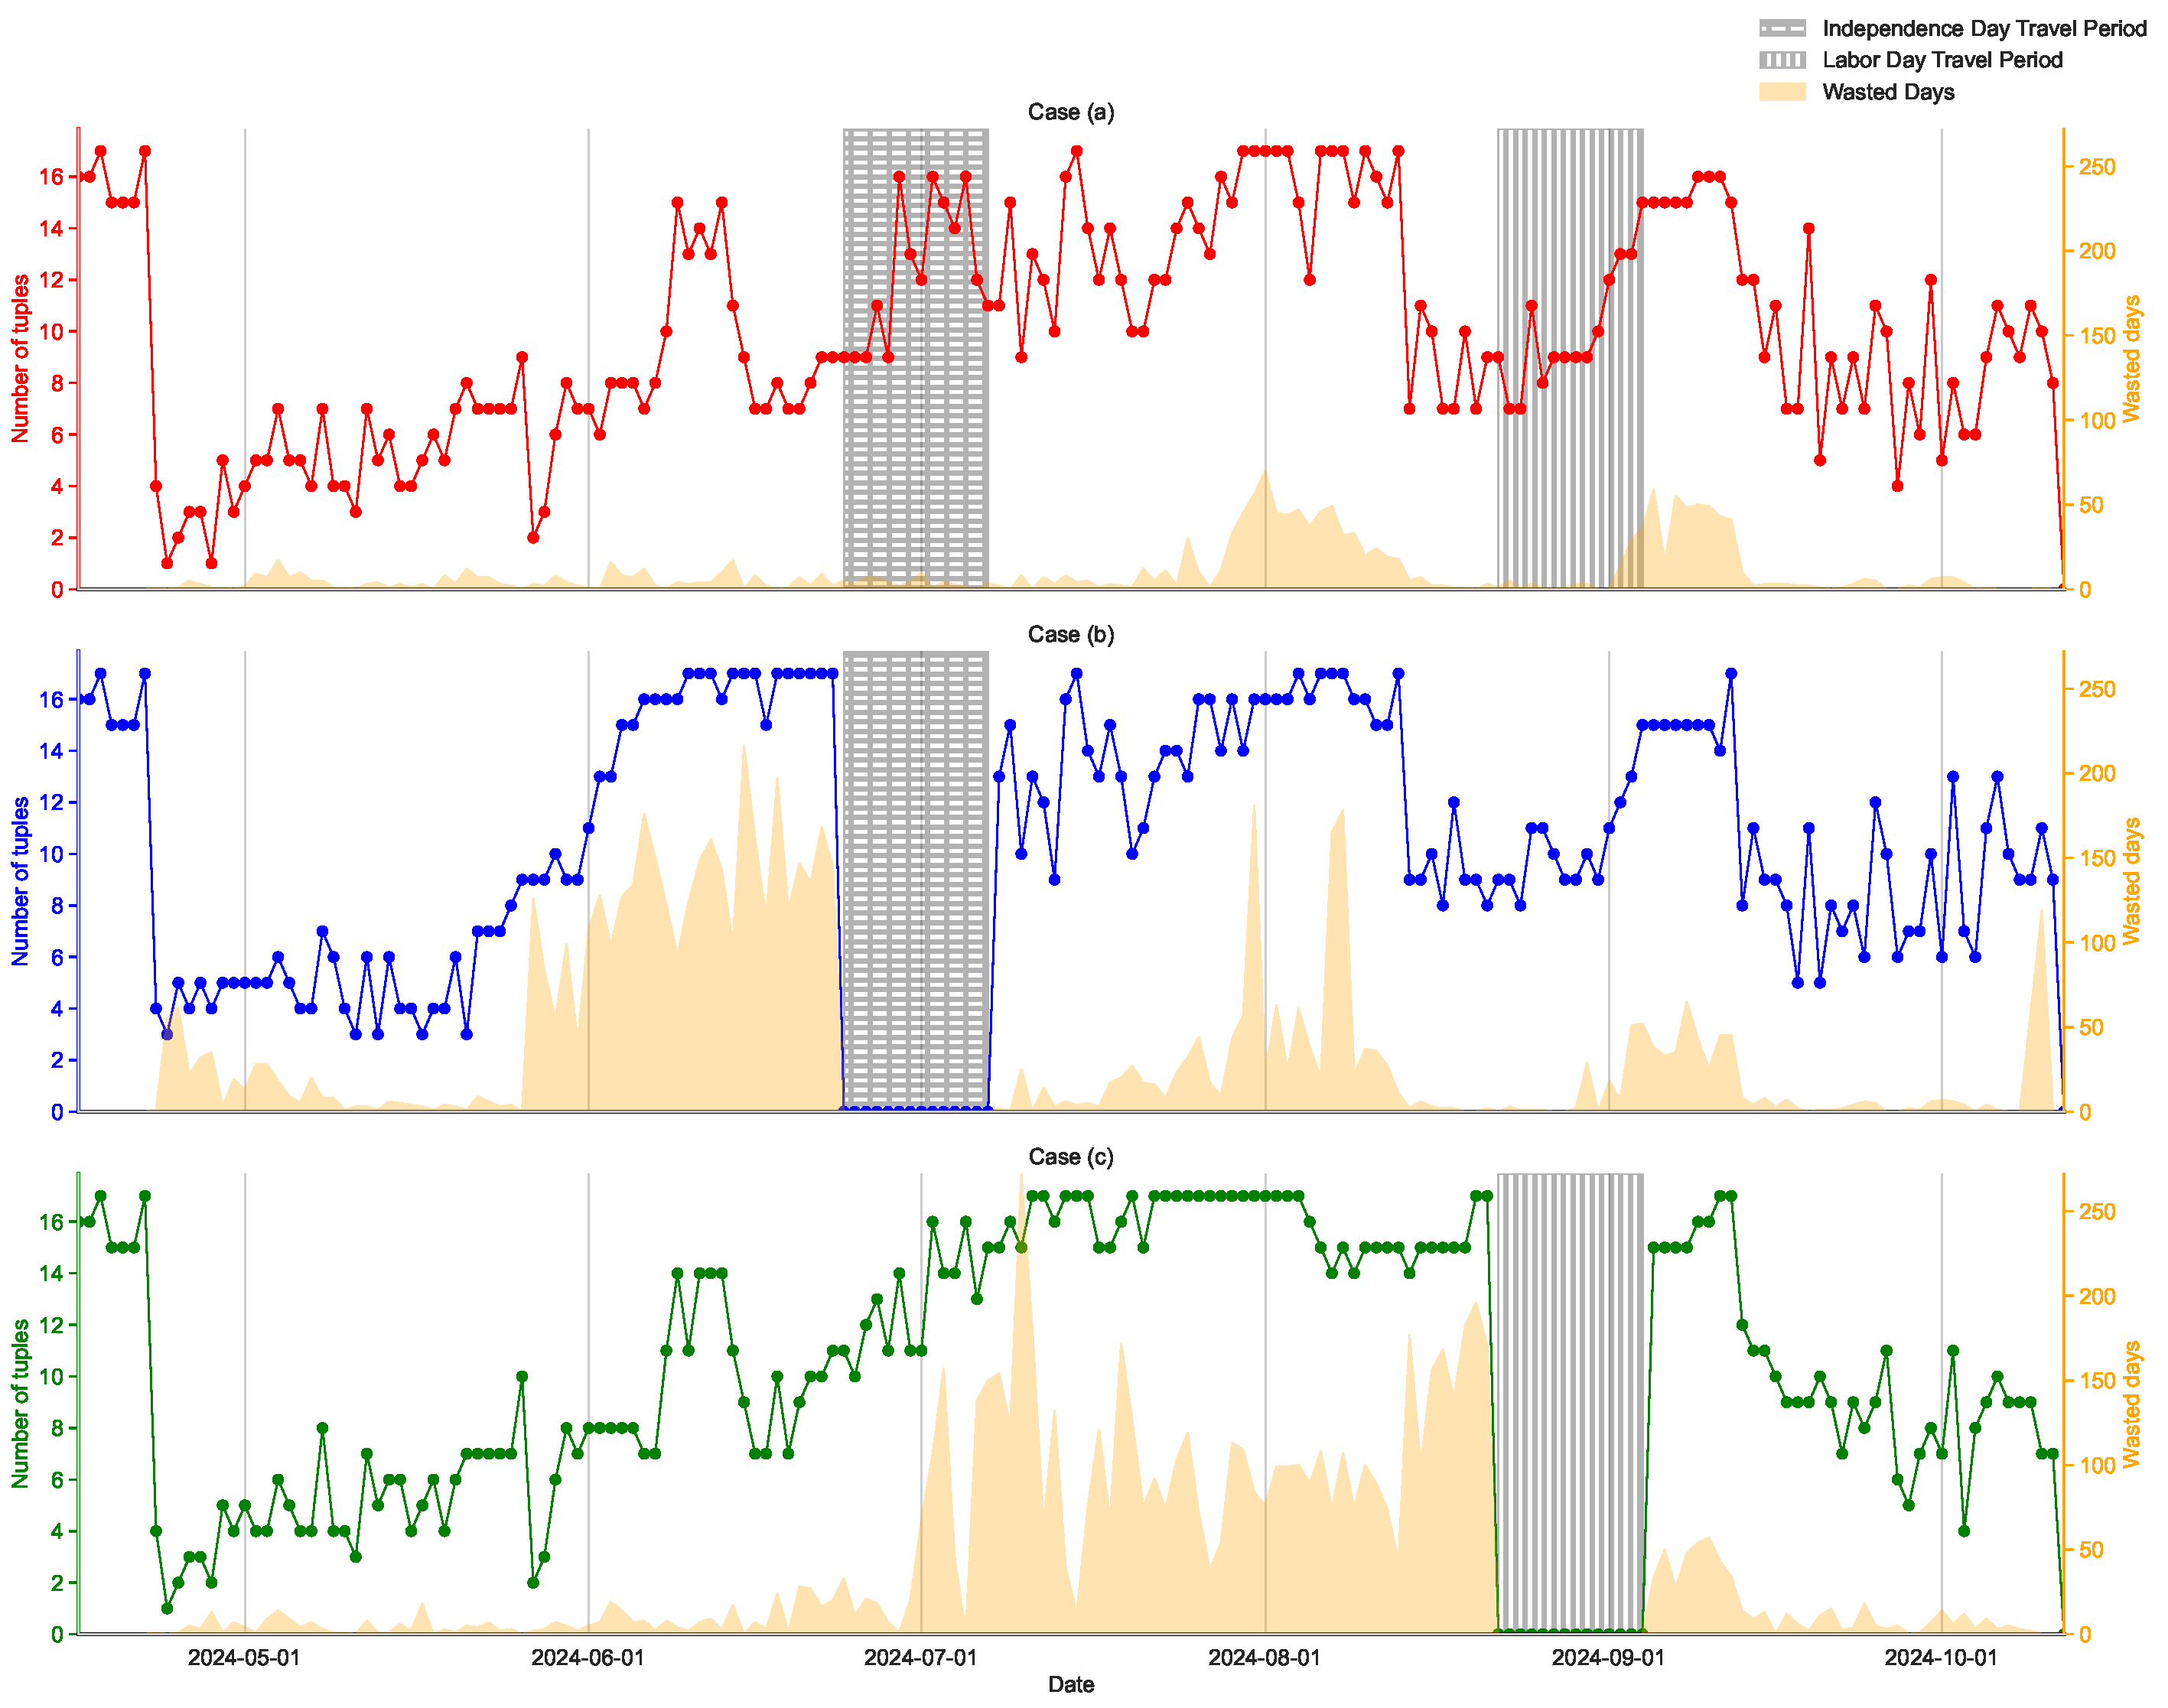
\includegraphics[width=\linewidth]{Effect_hol_red_v1.pdf}
    \caption{Effect of reduced station access during a two-week-long holiday travel period}
    \label{fig:effect_holiday_reduction}
\end{figure}

Figure~\ref{fig:effect_holiday_reduction} shows the number of scheduled tuples by day for each of the following three scenarios: (a) without any station access reductions, (b) with station access reductions only during the Independence Day travel period, and (c) with station access reductions only during the Labor Day travel period. For either holiday travel period, we observe that a large number of maintenance checks are conducted prematurely, in anticipation of the zero station access during the holiday travel period. Those premature maintenance checks imply significant economic costs. For tuple $w$, if maintenance is conducted  one day earlier than the due date (meaning that the DTG on the day of maintenance is two), the economic loss is estimated as $\frac{c_w}{m_w}$, where $c_w$ is the one-time maintenance cost for tuple $w$. Assuming that a C-Check costs \$250,000 \citep{ackert2010basics} and is good for 100 days, the economic loss of premature maintenance by a single day is thus \$2,500. Based on the wasted days visualized in Figure~\ref{fig:effect_holiday_reduction}, one can estimate the economic impact of closing maintenance stations in a travel peak period.


Table~\ref{tab-impact_sta_redu}  quantifies these impacts,  showing that due to the lack of station access during the holiday travel period, the weighted maintenance cost (namely the optimization objective) increases by 5.7\% for Independence Day and 6.1\% for Labor Day. As discussed in Section~\ref{performance_decomp}, those substantial percentage changes indicate significant wasted maintenance days. For instance, for the Labor Day travel period, the total number of wasted days across the entire fleet increases from 1,618  days to 6,595 days by 307.6\% or from approximately 0.9 days to 3.7 days per scheduled check. Another related metric also measures the significant impact of the holiday shut down on maintenance schedules. Table~\ref{tab-impact_sta_redu} shows that the average yield drops by 2.3\% and 3.6\% for the Independence Day and Labor Day, respectively. Given the above analyses of several key metrics, we conclude that the lack of station access during the Labor Day travel period has a larger impact on the maintenance plans. This also implies that if maintenance stations need to be closed for any reasons (such as for renovation), they should be closed during the Independence Day period rather than the Labor Day period to mitigate the impact on aircraft maintenance activities.

\begin{table}[htbp]
\centering
\caption{Impact of station access reductions during holiday travel periods on maintenance operations}
\label{tab-impact_sta_redu}
\resizebox{0.9\columnwidth}{!}{%
\begin{tabular}{@{}lccccc@{}}
\toprule
Cases & Objective value & \begin{tabular}[c]{@{}c@{}}$\%$ of premature \\ checks \end{tabular} & \begin{tabular}[c]{@{}c@{}}Total \\ wasted days\end{tabular} & \begin{tabular}[c]{@{}c@{}}Av. premature \\ days\end{tabular} & Av. yield \\ \midrule
Case (a) & 842.1 & 29.1$\%$ & 1,618 & 0.9& 99.1$\%$ \\
Case (b) & 889.9 & 44.1$\%$ & 6,087 & 3.4 & 96.7$\%$ \\
Case (c) & 893.1 & 48.3$\%$ & 6,595 & 3.7 & 95.4$\%$ \\ \bottomrule
\end{tabular}%
}
\end{table}


\subsection{Managerial Insights}
The case studies presented earlier yield the following important managerial insights:

\begin{enumerate}
    \item \textbf{Necessity and benefit of joint optimization.} Due to the close interrelationship between scheduling and station assignment decisions, each major airline with multiple spatially distributed maintenance bases finds it essential to jointly determine when and where to conduct maintenance for each aircraft. The joint decision-making has also been shown to be more advantageous, given its lower overall maintenance cost than the scheduling-first-assignment-second approach.
    \item \textbf{Impact of maintenance capacity.} Computational experiments indicate that when maintenance capacity is ample, airlines can schedule checks very close to their due dates to achieve almost perfect yields. By contrast, when capacities are tightly constrained, suboptimal and premature maintenance plans result. These findings suggest that aircraft maintenance operations managers should proactively manage maintenance facility capacities considering the maintenance demand of their fleets. 
    \item \textbf{Efficiency of the proposed decomposition strategies.} Although both proposed solution approaches have been proven effective, we note that the temporal decomposition approach should be appealing to aircraft maintenance planners in practice, especially considering its ease of implementation. To ensure successful implementation, two key time parameters of the rolling horizon framework should be carefully selected, and aircraft rotation requirements must be checked appropriately when transitioning from one time horizon to another
\end{enumerate}

\color{black}

